%\documentclass[conference]{IEEEtran}
\documentclass[runningheads]{llncs}

%\newtheorem{theorem}{Theorem}
%\newtheorem{definition}{Definition}
%\newtheorem{lemma}[theorem]{Lemma}
%\newtheorem{proposition}[theorem]{Proposition}

\newcommand{\RS}[2]{\mathsf{RS}[#1,#2]}
\newcommand{\RSC}[3]{\mathsf{RS}[#1,#2,{\bm{#3}}]}
\newcommand{\rsc}[2]{\mathsf{RS}_{\bm{#1}}[#2]}
\newcommand{\KK}{\mathbb{K}}
\newcommand{\HH}{\mathbb{H}}
\newcommand{\comm}{\mathsf{Com}}
\newcommand{\csetup}{\mathsf{Gen}}
\newcommand{\pip}{\mathsf{P}_\mathrm{ip}}
\newcommand{\vip}{\mathsf{V}_\mathrm{ip}}
\newcommand{\piplog}{\mathsf{P}_\mathrm{log}}
\newcommand{\viplog}{\mathsf{V}_\mathrm{log}}
\newcommand{\pipsq}{\mathsf{P}_\mathrm{sq}}
\newcommand{\vipsq}{\mathsf{V}_\mathrm{sq}}
\newcommand{\ip}{\mathrm{ip}}
\newcommand{\wit}{\mathsf{w}}
\newcommand{\ewit}{\mathsf{U}}
\newcommand{\setup}{\mathsf{S}}
\newcommand{\mc}[1]{\mathcal{#1}}
\newcommand{\innp}[2]{\langle #1,#2\rangle}
\newcommand{\innph}[2]{\bm{\langle\langle} #1,#2\bm{\rangle\rangle}} % hetero inner product
\newcommand{\matx}{\mathsf{X}}
\newcommand{\maty}{\mathsf{Y}}
\newcommand{\matz}{\mathsf{Z}}
\newcommand{\bi}{\mathsf{b}}
\newcommand{\wt}[1]{\mathbf{wt}({#1})}
\newcommand{\zcash}{\mathrm{Zcash}}
%\newcommand{\dec}{\mathsf{Dec}}

\newcommand{\rsoracle}{\mathcal{U}^{\mathsf{RS}}}
\newcommand{\comoracle}{\mathcal{O}} %^{\mathsf{Com}
\newcommand{\decode}{\mathsf{Dec}}
\newcommand{\dham}{\Delta}
\newcommand{\ric}[2]{\mathsf{RIC}(#1,#2)}
\newcommand{\cic}[2]{\mathsf{CIC}(#1,#2)}
\newcommand{\cbar}{\bar{\bm{c}}}
\newcommand{\aff}[2]{{\rm Aff}({#1},{#2})}
\newcommand{\bwit}{\overline{\mathsf{w}}}

\newcommand{\proximityTwoD}{\mathsf{Membership2D}}
\newcommand{\proximityThreeD}{\mathsf{Proximity3D}}
\newcommand{\rowInterleaved}{\mathsf{RowInterleavedTest}}
\newcommand{\colInterleaved}{\mathsf{ColumnInterleavedTest}}
\newcommand{\innerproduct}{\mathsf{InnerProduct}}
\newcommand{\linearcheck}{\mathsf{LinearCheck}}
\newcommand{\quadcheck}{\mathsf{QuadraticCheck}}
\newcommand{\grapheneRCS}{\mathsf{GrapheneR1CS}}
\newcommand{\agginnerproduct}{\mathsf{AggInnerProduct}}
\newcommand{\distproxTwoD}{\mathsf{DistMembership2D}}
\newcommand{\distproxThreeD}{\mathsf{DistProximity3D}}
\newcommand{\distlinearcheck}{\mathsf{DistLinearCheck}}
\newcommand{\distquadcheck}{\mathsf{DistQuadraticCheck}}
\newcommand{\dashL}{L^{+}}
\newcommand{\dashD}{d^{+}}
\newcommand{\linearcheckTwoD}{\mathsf{LinearCheck2D}}
\newcommand{\quadcheckTwoD}{\mathsf{QuadraticCheck2D}}
\newcommand{\proxcheckTwoD}{\mathsf{ProximityCheck2D}}
\newcommand{\fft}{\mathsf{FFT}}
\newcommand{\ifft}{\mathsf{IFFT}}
\newcommand{\cfft}{\mathsf{C}_\mathsf{FFT}}
\newcommand{\cmexp}{\mathsf{C}_\mathsf{MXP}}
\newcommand{\cexp}{\mathsf{C}_\mathsf{EXP}}
\newcommand{\cfop}{\mathsf{C}_\mathbb{F}}
\newcommand{\bitsF}{\mathsf{B}_\mathbb{F}}
\newcommand{\bitsG}{\mathsf{B}_\mathbb{G}}
\newcommand{\open}{\mathsf{Open}}
\newcommand{\w}{\omega}
\newcommand{\IF}[1]{\calF_{#1}}
\newcommand{\zetabar}{\overline{\bm{\zeta}}}
\newcommand{\etabar}{\overline{\bm{\eta}}}


% 		Notations for DPZK

\newcommand{\prrounds}{r_\mathsf{pr}}
\newcommand{\prcomm}{c_\mathsf{pr}}
\newcommand{\zkrounds}{r_\mathsf{zk}}
\newcommand{\zkcomm}{c_\mathsf{zk}}



% 		Calligraphic and blackboard type letters.

\def\cA{{\calA}}
\def\cB{{\calB}}
\def\cC{{\calC}}
\def\cD{{\calD}}
\def\cE{{\calE}}
\def\cF{{\calF}}
\def\cG{{\calG}}
\def\cH{{\calH}}
\def\cI{{\calI}}
\def\cJ{{\calJ}}
\def\cK{{\calK}}
\def\cL{{\calL}}
\def\cM{{\calM}}
\def\cN{{\calN}}
\def\cO{{\calO}}
\def\cP{{\calP}}
\def\cQ{{\calQ}}
\def\cR{{\calR}}
\def\cS{{\calS}}
\def\cT{{\calT}}
\def\cU{{\calU}}
\def\cV{{\calV}}
\def\cW{{\calW}}
\def\cX{{\calX}}
\def\cY{{\calY}}
\def\cZ{{\calZ}}
\def\cq{{\calq}}
%%%%%%%%%%%%%%%%%
\def\bbC{{\mathbb C}}
\def\bbE{{\mathbb E}}
\def\bbF{{\mathbb F}}
\def\bbG{{\mathbb G}}
\def\bbM{{\mathbb M}}
\def\bbN{{\mathbb N}}
\def\bbQ{{\mathbb Q}}
\def\bbR{{\mathbb R}}
\def\bbV{{\mathbb V}}
\def\bbZ{{\mathbb Z}}

\def\Zq{\bbZ_q}

%%%%%%%%%%%%%%%%%

\def\calA{\mathcal{A}}
\def\calB{\mathcal{B}}
\def\calC{\mathcal{C}}
\def\calD{\mathcal{D}}
\def\calE{\mathcal{E}}
\def\calF{\mathcal{F}}
\def\calG{\mathcal{G}}
\def\calH{\mathcal{H}}
\def\calI{\mathcal{I}}
\def\calJ{\mathcal{J}}
\def\calK{\mathcal{K}}
\def\calL{\mathcal{L}}
\def\calM{\mathcal{M}}
\def\calN{\mathcal{N}}
\def\calO{\mathcal{O}}
\def\calP{\mathcal{P}}
\def\calQ{\mathcal{Q}}
\def\calR{\mathcal{R}}
\def\calS{\mathcal{S}}
\def\calT{\mathcal{T}}
\def\calU{\mathcal{U}}
\def\calV{\mathcal{V}}
\def\calW{\mathcal{W}}
\def\calX{\mathcal{X}}
\def\calY{\mathcal{Y}}
\def\calZ{\mathcal{Z}}
\def\calq{\mathcal{q}}

\def\bbA{\mathbb{A}}
\def\bbB{\mathbb{B}}
\def\bbC{\mathbb{C}}
\def\bbD{\mathbb{D}}
\def\bbE{\mathbb{E}}
\def\bbF{\mathbb{F}}
\def\bbG{\mathbb{G}}
\def\bbH{\mathbb{H}}
\def\bbI{\mathbb{I}}
\def\bbJ{\mathbb{J}}
\def\bbK{\mathbb{K}}
\def\bbL{\mathbb{L}}
\def\bbM{\mathbb{M}}
\def\bbN{\mathbb{N}}
\def\bbO{\mathbb{O}}
\def\bbP{\mathbb{P}}
\def\bbQ{\mathbb{Q}}
\def\bbR{\mathbb{R}}
\def\bbS{\mathbb{S}}
\def\bbT{\mathbb{T}}
\def\bbU{\mathbb{U}}
\def\bbV{\mathbb{V}}
\def\bbW{\mathbb{W}}
\def\bbX{\mathbb{X}}
\def\bbY{\mathbb{Y}}
\def\bbZ{\mathbb{Z}}

\def\sfR{\mathsf{R}}
%%%%%%%%%%%%%%%%%%%%%%%%%


% 		Rounding commands

%\newcommand{\ceil}[1]{\left\lceil #1 \right\rceil}
%\newcommand{\floor}[1]{\left\lfloor #1 \right\rfloor}
\newcommand{\round}[1]{\left\lfloor #1 \right\rceil}

%%%%%%%%%%%%%%%%%

% 		Algorithms
\def\dpzk{\mathsf{DPZK}}
%\def\dfzk{\mathsf{dfzk}}
\def\Exec{\mathsf{Exec}}
\def\Setup{\mathsf{Setup}}
\def\View{\mathsf{View}}
\def\Num{\mathsf{N}} % number of provers
\def\wit{\mathsf{w}} %Witness
\def\extwit{{w}} %Extended witness
\def\stmt{{x}} %Statement
\def\prover{\mathcal{P}} %Prover
\def\verifier{\mathcal{V}} %Verifier
\def\ppt{\mathsf{PPT}}
\def\extr{\mathcal{E}} %Extractor
\def\extrac{\extr} %Extractor
\def\DPZK{\text{DPZK}}
\def\Sim{\mathcal{S}} %Simulator
\def\bitset{\{0,1\}} %{0,1}
\def\intpartofC{\mathsf{M}} %Interactive part of the circuit
\def\gen{\mathsf{Gen}} %Gen
\def\com{\mathsf{Com}} %commitment
\def\pccom{\mathsf{pcCom}} %product codeword commitment
\def\ocom{\mathsf{oCom}} %oracle commitment
\def\NP{\mathsf{NP}} %NP class
\def\C{\mathsf{C}} %Circuit
\def\round{\mathsf{R}} %Round
\def\tr{\mathsf{tr}} %Transcript
\def\RS{\mathsf{RS}}
\def\oracle{\mathcal{U}^{\RS}} %Oracle
\def\cm{\mathsf{cm}} %Commitment vector
%\def\Real{\mathsf{Real}} % Real world
\def\circsize{\mathsf{|C|}}
\def\Ag{\mathsf{A}} %Aggregator
\newcommand{\distprover}{\prover_\xi}
\newcommand{\combine}{\mathsf{Combine}}
\newcommand{\shr}[1]{\langle{#1}\rangle^\xi}
% 		Notions
\def\ZKUC{\mathsf{ZKUC}}

\def\negl{\mathrm{negl}}
\def\abort{\texttt{abort}}

\def\inp{\mathsf{in}}
\def\st{\mathsf{st}}
\def\secp{{\lambda}}

\newcommand{\pr}{\text{\em Pr}}
\newcommand{\Defn}[1]{\textbf{{\textit{#1}}}}
\newcommand{\Adv}{\mathcal{A}}

%\newcommand{\com}{\mathsf{com}}
\newcommand{\vc}[1]{\textbf{{#1}}}
%\newcommand{\bb}[1]{\mathbb{#1}}
%\newcommand{\poly}[1][2]{#1(#2)}
%\newcommand*{\poly}[1][2]{#1(#2)}
\newcommand{\qb}{q_{blind}}
\newcommand{\qbj}{q_{{blind}_j}}
\newcommand{\boldm}[1]{\mathversion{bold}#1\mathversion{normal}}
%\newcommand{\trans}[1]{\textbf{\tau_{#1}}}
\def\T{T} % Matrix T
\def\A{A} % Matrix A
\def\B{B} % Block B
\def\AT{A\cdot T} %Matrix A.T
\def\tc{\tilde{c}}
\def\tU{\widetilde{U}} 
\def\tv{\tilde{v}}
\def\vecx{\textbf{x}}
\def\oQ{\overline{Q}}
\def\oq{\overline{q}}
\def\oU{\overline{U}}
\def\q1b{q_{1_{blind}}}
\def\q1bj{q_{1_{blind_j}}}
\def\P{\textit{P}} %Prover
\def\V{\textit{V}} %Verifier
\def\vecx{$\textbf{\x}$}
\def\ctsize{N}

%----------Comments-----------
% Author notes
\def\ShowAuthNotes{1}
\ifnum\ShowAuthNotes=1
%\newcommand{\authnote}[2]{{\textbf{$\mathbf{\big[}$~#1's note:}} \textbf{\em\small #2}~{$\mathbf{\big]}$}}
\newcommand{\authnote}[2]{\\ \textcolor{red}{\parbox{0.9\linewidth}{[{\footnotesize {\bf #1:} { {#2}}}]}}\\}
\newcommand{\pnote}[1] {\textcolor{red}  {[PKP:{\sl{#1}}]}}
\newcommand{\commentA}[1]{\textcolor{cyan}{{\sf (Arpita's Note:} {\sl{#1}} {\sf EON)}}}
\else
\newcommand{\authnote}[2]{}
\newcommand{\pnote}[1] {}
\newcommand{\commentA}[1]{}
\fi

\newcommand{\dnote}[1]{\authnote{VD}{#1}}
%\newcommand{\pnote}[1]{\authnote{PKP}{#1}}
\newcommand{\nnote}[1]{\authnote{NS}{#1}}
\newcommand{\pdnote}[1]{\authnote{PD}{#1}}



	\newcommand{\Func}{\mathcal{F}}
%	\newcommand{\Env}{\mathcal{Z}}
	\newcommand{\Ideal}{\ensuremath{\textsc{ideal}}}
	\newcommand{\Real}{\ensuremath{\textsc{real}}}
	\newcommand{\Hyb}{\ensuremath{{\textsc{hyb}}}}
%	\newcommand{\NN}{\mathbb{N}}
	\newcommand{\FSA}{\ensuremath{\mathcal{F}_{\mathsf{sa}}}}
	\newcommand{\FDPZK}{\ensuremath{\mathcal{F}_{\mathsf{dpzk}}}}
%	\newcommand{\FF}{\ensuremath{\mathcal{F}_{\mathsf{fair}}}}
	\newcommand{\FG}{\ensuremath{\mathcal{F}_{\mathsf{god}}}}
	\newcommand{\FA}{\ensuremath{\mathcal{F}_{\mathsf{ua}}}}
	\newcommand{\Partyset}{\mathcal{P}}
	\newcommand{\bit}{\{0,1\}}
\newenvironment{boxfig}[2]{% {#1}{#2} = {Caption}{label}
     \begin{figure}[htb!]
     \newcommand{\FigCaption}{#1}
     \newcommand{\FigLabel}{#2}
       \vspace{-.15cm}
     \begin{center}
       \begin{small}
         \begin{tabular}{@{}|@{~~}l@{~~}|@{}}
           \hline
           %\rule[-1ex]{0pt}{1ex}\begin{minipage}[!htb]{\textwidth}   
            \rule[-1.5ex]{0pt}{1ex}\begin{minipage}[b]{\linewidth}
             \vspace{1ex}
             \smallskip
             }{%
           \end{minipage}\\
           \hline
         \end{tabular}
       \end{small}
        \vspace{-0.3cm}
       \caption{\FigCaption}
       \figlab{\FigLabel}
     \end{center}
     \vspace{-.5cm}
   \end{figure}
}


\title{Zero-Knowledge Proof Systems with Distributed Proof Generation}
%\author{\IEEEauthorblockN{Protik}}
\begin{document}
\tikzstyle{line} = [draw,-latex']
\tikzstyle{block}=[draw, rectangle]
\maketitle

\begin{abstract}

Traditional zero-knowledge protocols have been studied and optimized for the setting where a single prover holds the complete witness and trying to convince a verifier about a predicate on the witness, without revealing any additional information to the verifier. This work initiates the study of distributed proof generation where the witness is shared among multiple mutually distrusting provers and they want to convince a verifier that their shares together satisfies the predicate. We start by defining a new MPC-style security definition to capture the possible adversarial settings, and proposing new efficiency parameters for distributed proof generation on the number of rounds $\prrounds$ and the amount of communication $\prcomm$ among the provers. Next, we propose a new zero-knowledge protocol \name{} in the Interactive Probabilistically Checkable Proofs (IPCP) paradigm which admits $O(N^{1/c})$ proof size. The provers in \name{} have a total communication complexity $O(\Num \cdot N^{1-2/c}+ N)$ when the proof is generated distributively among $\Num$ provers.


%=======
%Traditional zero-knowledge protocols have been studied and optimized for the setting where a single prover holds the complete witness and trying to convince a verifier about a predicate on the witness, without revealing any additional information to the verifier. This work initiates the study of distributed proof generation where the witness is shared among multiple mutually distrusting provers and they want to convince a verifier that their shares together satisfies the predicate. We start by defining a new MPC-style security definition to capture the possible adversarial settings, and proposing new efficiency parameters for distributed proof generation on the number of rounds $\prrounds$ and the amount of communication $\prcomm$ among the provers. We then propose a new zero-knowledge protocol \name{} in the IPCP paradigm which admits $O(N^{1/c})$ proof size. The provers in \name{} have a total communication complexity $O(\Num \cdot N^{1-2/c}+ N)$ when the proof is generated distributively among $\Num$ provers.
%>>>>>>> 393208ba0fc46c06f17b37a8cad4e0128ff8bbf5
%\end{comment}
%	Zero knowledge is an intriguing area of research from the prospect of theory as well as application, where a party, prover \textit{P}, tries to convince verifier \textit{V} that a statement $x$( instance of an NP language) is correct using a witness $w$ such that $M(x,w)=1$. Let $C$ be the circuit representation of $M$ and $|C|$ is the size of $C$ i.e. the no. of gates in $C$. The work of Ligero in this problem proposed a solution where proof size is $O(|C|^{1/2})$. They solve the problem by converting a NP language to it's corresponding circuit satisfiability problem. $w\in \mathbb{F}^{ml}$ be the extended witness which is the secret input to the prover. Prover \textit{P} encodes $w$ to a matrix $U$ of size $m\times n$, where $m, n, l = O(\sqrt{|C|})$ and $n>l$. In Ligero's protocol first check is for to ensure that the matrix $U$ is a correct encoding, that is done by testing interleaved. Then they check that all the outcomes of all the gates( addition and multiplication) are correct or not, and to do that they introduce two checks, linear constraint and quadratic constraint. We are using the same approach of Ligero, but our encoding is different. Instead of matrix we will encode $w$ to a box( matrix of 3 dimensions), to keep the familiarity of notation we will consider $w\in \mathbb{F}^{pml}$ and the size of the box $U$ is $p\times m\times n$, where $p, m, n, l = O(\sqrt[3]{|C|})$ and $n>l$. To encode $w$ we are going to construct $pm$ many polynomials(univariate) such that each of them has degree at most $s$, where $s$ is some suitable number between $l$ and $n$. 
%\\

%\mycomment{Adding a version below.}
%The work of Ligero[citation] proposed ... In Ligero, a witness $x$ is encoded into a matrix $U$ of dimension $m \times n$, where $m$ and $n$ denote - and - respectively. Our idea is similar to theirs apart from the witness being encoded to a {\em box}. A box is a 3-dimensional matrix ($m \times n \times p$) where --(add technical details of box here). This ensures linearity of (what?) along both rows and columns. We hope that the aforementioned encoding along with homomorphic commitments lead to a ZK proof, whose size will be $O(|C|^{\frac{1}{3}})$.
\end{abstract}

%Let $x$ be the witness which encoded to $U$ where $m$ is the no. of rows, $n$ is the no. of columns in a slice (one vertical matrix), and there are $p$ many slices.\\
%Initially consider $m=n$\\


\section{Preliminaries}\label{sec:prelims}
\subsection{Linear Codes}
\begin{definition}\label{defn:lincode}
.\commentA{this looks like general definition for code. why is it called linear? change}
For positive integers $n,k$ and a finite field $\bbF$, a $k$-dimensional linear subspace $L$ of $\bbF^n$ is called an $[n,k]$ linear code. Elements of $L$ are conventionally called {\em codewords}. 
\end{definition}

For codewords $x,y\in L$ where $x=(x_1,\ldots,x_n)$ and $y=(y_1,\ldots,y_n)$ we define the hamming distance $\dham(x,y)=|\{i\in [n]: x_i\neq y_i\}|$. It is easily checked that $\dham$ defines a metric on $L$. The minimum distance of the code $L$, denoted by $\delta(L)$ is defined as $\min\{\dham(x,y):x,y\in L, x\neq y\}$.

For an $[n,k]$ code $L$, a $n\times k$ matrix $\calG$ is called a {\em generator matrix} iff (i) $\calG x\in L$ for all $x \in \bbF^k$ and (ii) $\calG x\neq \calG y$ for $x\neq y$. Clearly, such a matrix $\calG$ has rank $k$. Similarly an $n\times (n-k)$ matrix $\calH$ such that $y^T \calH = 0$ for all $y\in L$ is called a {\em parity check} matrix for $L$. It is easily seen that the above two matrices exist for any $[n,k]$ linear code $L$. We will assume that description of the linear code $L$ includes a generator matrix $\calG$ and a parity check matrix $\calH$.

\begin{definition}[Interleaved Code]\label{defn:interleavedcode}
For an $[n,k]$-linear code $L$ and a positive integer $m$, we define a {\em row interleaved code} $\ric{L}{m}$ to be the set of $m\times n$ matrices $A$ such that each row of $A$ is a codeword in $L$. Similarly, we define a {\em column interleaved code} $\cic{L}{m}$ to be the set of $n\times m$ matrices $B$ such that each column of $B$ is a codeword in $L$.
\end{definition}

For a linear $[n,k]$-code $L$ over the field $\bbF$, we observe that $\ric{L}{m}$ forms an $[n,k]$-code over the field $\bbF^m$ by viewing each column of the codeword $A\in \ric{L}{m}$ as an element in the field $\bbF^m$ \commentA{this isn't clear at all }. Similarly, $\cic{L}{m}$ forms an $[n,k]$ code over $\bbF^m$ by viewing each row of the codeword $B\in \cic{L}{m}$ as an element in $\bbF^m$. For $A,A'\in \ric{L}{m}$, we define the distance $\dham(A,A')=|\{i\in [n]: A[\cdot,i]\neq A'[\cdot,i]\}|$ where the notation $X[\cdot,i]$ denotes the $i^{th}$ column of the matrix $X$. Similarly for $B,B'\in \cic{L}{m}$ we define $\dham(B,B')=|\{i\in [n]: B[i,\cdot]\neq B'[i,\cdot]\}|$.
 
\begin{definition}[Product Code]\label{defn:productcode}
Let $L_i$ be an $[n_i,k_i]$-linear code for $i=1,2$. We define the product code $L_1\otimes L_2$ \commentA{bad notation for product code; better now? } to be the code consisting of $n_2\times n_1$ matrices $A$ such that each row of $A$ is a codeword in $L_1$ and each column of $A$ is a codeword in $L_2$. 
\end{definition}

Note that by definition, the product code $L_1\otimes L_2$ is a row interleaved code of $L_1$ and a column interleaved code of $L_2$, i.e $L_1\otimes L_2 =
\ric{L_1}{n_2}\cap \cic{L_2}{n_1}$. For $A,A'\in L_1\otimes L_2$, we define $\dham_1(A,A')=|\{i\in [n_1]: A[\cdot,i]\neq A'[\cdot,i]\}|$ and $\dham_2(A,A')=|\{i\in
[n_2]: A[i,\cdot]\neq A'[i,\cdot]\}|$. The distance $\dham_1$ corresponds to distance function of the code $\ric{L}{n_2}$, where we view $A,A'$ as codewords in $\ric{L}{n_2}$. Similarly, the distance $\dham_2$ corresponds to the distance function of the code $\cic{L}{n_1}$.
\commentA{where is the proof for existence of such code?}

\begin{definition}[Reed Solomon Code]\label{defn:rscode}
An $[n,k]$-Reed Solomon Code $L\subseteq \bbF^n$ consists of vectors $(p(\eta_1),\ldots,p(\eta_n))$ for polynomials $p\in \bbF[x]$ of degree less than $k$ where $\eta_1,\ldots,\eta_n$ are distinct points in $\bbF$. We will use $\rsc{\eta}{k}$ to denote the Reed Solomon code with $\bm{\eta}=(\eta_1,\ldots,\eta_n)$ and $deg(p)<k$.
\end{definition}

\begin{lemma}\label{lem:bicdecoding}
Let $L_1 := \rsc{\eta}{\ell}$ and $L_2 := \rsc{\alpha}{m}$ be $[n,\ell]$ and
$[h,m]$ Reed Solomon codes respectively. Let $\mc{C}_1 := \ric{L_1}{h}$ and
$\mc{C}_2 := \cic{L_2}{n}$ be the interleaved codes of $L_1$ and $L_2$. Suppose
a matrix $U^\ast\in \FF^{h\times n}$ satisfies $d_1(U^\ast,\mc{C}_1)<e_1$ and
$d_2(U^\ast,\mc{C}_2)<e_2$ for $e_1\leq n-\ell$ and $e_2\leq h-m$\commentA{what are $d_1$ and $d_2$? These are never defined. }. Then, there exists $U\in L_1\otimes L_2$ and sets
$S_1\subseteq [n]$, $S_2\subseteq [h]$ with $|S_1|>n-e_1$ and $S_2>h-e_2$ such
that $U^\ast[i,j]=U[i,j]$ for $(i,j)\in S_1\times S_2$.
\commentA{where is the proof?}
\end{lemma}

\begin{proof}
	Let $U_1 \in \mc{C}_1$  such that $\dham_1(U^\ast, U_1) \leq \dham(U^\ast, U) \forall U\in \mc{C}_1$ and let $\dham_1(U^\ast, U_1) = \beta_1$ with $\beta_1<e_1$
	Therefore $U^\ast$ differs from $U_1$ in $\beta_1$ many columns, i.e. in the remaining $n-\beta_1$ columns $U^\ast$ and $U_1$ are identical.
	So, there are columns $S_1 = \{j_{s} : s\in [n - \beta_1] \}$ for which $U^\ast[i,j] = U_1[i,j]$ $\forall j\in S$.
	Let $U_2 \in \mc{C}_2$  such that $\dham_2(U^\ast, U_2) \leq \dham(U^\ast, U) \forall U\in \mc{C}_2$ and let $\dham_1(U^\ast, U_2) = \beta_2$ with $\beta_2<e_2$
	Therefore $U^\ast$ differs from $U_2$ in $\beta_2$ many rows, i.e. in the remaining $n-\beta_1$ rows $U^\ast$ and $U_2$ are identical.
	So, there are rows $S_2 = \{i_{t} : t\in [h - \beta_2] \}$ for which $U^\ast[i,j] = U_2[i,j]$ $\forall i\in T$.
	
	$U_1\in \mc{C}_1 \implies \exists$ polynomials $p_1(\cdot), \ldots, p_h(\cdot)$ of degree $< \ell$
	
	$U_2\in \mc{C}_2 \implies \exists$ polynomials $q_1(\cdot), \ldots, q_n(\cdot)$ of degree $< m$
	
	Such that $p_i(\eta_j) = U_1[i,j] \& q_i(\alpha_j) = U_2[j,i]$
	
	Therefore, $U_1[i,j] = U_2[i,j]$ $\forall i\in S_1, j\in S_2$. Choose a bivariate polynomial $Q(x,y)$ such that $deg_x(Q)<\ell $ and $deg_y(Q)<m$ and $Q(\eta_{i_s}, \alpha_{j_t}) = U_1[i_s,j_t] = U_2[i_s,j_t] \forall (i, j)\in S_1\times S_2$. 
	
	Defne $U = Q(\eta_i,\alpha_j)$ $\forall i\in[h], j\in[n]$, Then $U \in \L_1\otimes L_2$ and $U^\ast[i,j] = U[i,j]$ $\forall (i,j) \in S_1 \times S_2$.
	
	And $|S_1|= n-\beta_1 > n-e_1$ and $|S_2|= h-\beta_2 > h-e_2$.
	This proves the above claim.	
\end{proof}
 

\subsection{Geometric Results on Linear Codes}
In this section, we prove some ``geometric'' results about subspaces spanned by linear codes. 
These results will play a key role in protocols for checking that the witness has been correctly encoded with small query complexity. Some variants of results presented in this section appear as lemmas and conjectures in \cite[Section 4]{ligero}.

Throughout this section, let $L$ be a linear $[n,k,d]$ code over field a finite $\HH$ and let $\FF\subseteq \HH$ be a subfield.  Let $m\geq 1$ be an integer, and let $\mc{C}$ denote the row interleaved code $\ric{L}{m}$. For a matrix $U\in \HH^{m\times n}$ and a vector $u_0\in \HH^n$, let $\aff{u_0}{U}$ denote the affine space given by:
\begin{equation}\label{eq:affspace}
\aff{u_0}{U} := \{u_0+r^TU: r\in \FF^m\}
\end{equation}
Note that in the above, the scalars in the linear combination come from $\FF$.

\begin{lemma}\label{lem:farpoint}
Let $L$ and $\mc{C}$ be codes as defined, and let $e$ be a positive integer such that $e+2\leq |\FF|$. Then for any $u_0\in \HH^n$ and any $U^\ast\in \HH^{m\times n}$ such that $d(U^\ast,\mc{C})>e$, there exists $v\in \aff{u_0}{U^\ast}$ such that $d(v,L)>e$.
\end{lemma} 
\begin{proof}
For sake of contradiction, assume that $d(u,L)\leq e$ for all $u\in
\aff{u_0}{U^\ast}$. Let $x$ be the point in $\aff{u_0}{U^\ast}$ such that
$d(x,L)$ is maximum. By assumption $d(x,L)\leq e$. Let $v\in L$ be such that
$\Delta(x,v)=d(x,L)$. Let $E\subseteq [n]$ be the set of positions where $x$ and
$v$ differ. Since $d(U^\ast,\mc{C})>e$, there exists row $R$ of $U^\ast$ and
position $j\in [n]$ 
such that $R_j\neq 0$.\pnote{Is this for all $j\in[n]$ or $\exists j\in [n]$? Why this is true?} Let
$\alpha_1,\ldots,\alpha_{e+1}$ be distinct non zero elements in $\FF$. Let $E_k$
for $k=1,\ldots,e+1$ denote the set of positions where $x+\alpha_kR$ and $v$
differ. Fix a position $i\in E$. Then there exists at most one $k\in [e+1]$ such
that $i\not\in E_k$. By pegion hole principle, there exists $k\in [e+1]$ such
that $E\subseteq E_k$. We also observe that since $\alpha_k\neq 0$, $j\in E_k$.
Thus $d(x+\alpha_k,v)>d(x,v)$, contradicting the choice of $x$. This proves the
lemma.   
\end{proof}


\begin{lemma}[Affine Line]\label{lem:affineline}
Let $L$ be the linear code as defined. Define an affine line $\ell_{u,v}$ in $\HH^n$ as $\ell_{u,v} := \{u + \alpha v:\alpha\in \FF\}$ for $u,v\in \HH^n$. Then for $e < d/3$ and any affine line $\ell_{u,v}$ we have:
\begin{enumerate}[{\rm (i)}]
\item $d(x,L)\leq e$ for all $x\in \ell_{u,v}$, or
\item $d(x,L)> e$ for at most $d$ points in $\ell_{u,v}$.
\end{enumerate}
\end{lemma}
We defer the proof of the above lemma to Appendix.
The next result underlies our key proximity protocols. Intuitively the result states that if a matrix is far away from the code $\mc{C}$, a random linear combination of its rows is far away from a codeword in $L$, and thus the proximity of the matrix to $\mc{C}$ may be tested by testing the proximity of a random linear combination of its rows to $L$.

\begin{lemma}[Affine Subspace]\label{lem:affinesubspace}
Let the codes $L$ and $\mc{C}$ be as defined and $e<d/3$ be an integer. Let $U\in \HH^{m\times n}$ be a matrix such that $d(U,\mc{C})>e$. Then for any $u_0\in \HH^n$, $\prob{d(u_0+r^TU,L)\leq e}\leq d/|\FF|$ for uniformly sampled $r\sample \FF^m$.
\end{lemma}
\begin{proof}
From Lemma \ref{lem:farpoint}, there exists $u\in \aff{u_0}{U}$ such that $d(u,L)>e$. Now we can write $\aff{u_0}{U}$ as union of affine lines passing through $u$. Applying lemma \ref{lem:affineline} to each line, we see that at most $d$ points $x$ on each affine line satisfy $d(x,L)\leq e$. Thus, a randomly sampled point $x$ in $\aff{u_0}{U}$, equivalently obtained as $u_0+r^TU$ for a randomly sampled vector $r\in \FF^m$ satisfies $d(x,L)$ with probability at most $d/|\FF|$.
\end{proof}

\noindent{\bf Three dimensional interleaving}: Consider a $p\times m\times n$ three dimensional
matrix $U[\cdot,\cdot,\cdot]$. We refer to $U[i,\cdot,\cdot]$ as $i^{th}$ {\em
slice}
of $U$, while we refer to $U[\cdot,\cdot,k]$ as the $k^{th}$ {\em plane} of $U$. Let $\mc{C}^p$ denote the set of $p\times m\times n$ matrices $U$ such that
each slice of $U$ is a codeword in $\mc{C}$. Let $\Delta_1$ denote the distance
metric on the set of $p\times m\times n$ matrices denoting the number of planes
where they differ, i.e, $\Delta_1(U,U')=|\{k\in [n]:
U[\cdot,\cdot,k]=U'[\cdot,\cdot,k]\}|$. \pnote{It should be $\neq$, right?} As before, define $d(U^\ast,\mc{C}^p)$ to be
the minimum value $\Delta_1(U^\ast,U)$ for $U\in \mc{C}^p$. The next result
states that if a three dimensional matrix $U$ is far away from the code
$\mc{C}^p$, a random linear combination of slices of $U$ is far away from $C$.

\begin{lemma}[3D Compression]\label{lem:3dcompression}
Let the codes $L,\mc{C}$ and $\mc{C}^p$ be as defined. Let $U^\ast$ be a
$p\times m\times n$ matrix such that $d(U^\ast,\mc{C}^p)>e$. Then for any
$m\times n$ matrix $u_0$, we have 
\[ \prob{d\left(u_0 + \sum_{i=1}^p r_iU^\ast[i,\cdot,\cdot], \mc{C}\right)\leq e}\leq
\frac{d}{|\FF|}\]  
for a uniformly sampled $(r_1,\ldots,r_p)\sample \FF^p$. 
\end{lemma}
\begin{proof}
Let $\HH$ denote the field $\FF^m$. Then $u_0$ can be viewed as a point in
$\HH^n$. Similarly $U$ can be viewed as $p\times n$ matrix over $\HH$.
We consider $\mc{C}$ as $[n,k,d]$ code over $\HH$ and $\mc{C}^p$ as the
interleaved code of $\mc{C}$ over the field $\HH$. Then by applying Lemma \ref{lem:affinesubspace}
with $\HH=\FF^m$ and codes $\mc{C}$ and $\mc{C}^p$ in place of codes $L$ and
$\mc{C}$, we have the desired bound.
\end{proof}


\subsection{Inner Product Arguments}
We define an interactive protocol that allows proving inner product relation over committed values. 
\begin{definition}\label{defn:commscheme}
 A pair of $\ppt$ algorithms $(\gen,\com)$ constitute a non-interactive commitment scheme if $\sigma\sample \gen(\secparam)$ consists of description of sets $\calM_\sigma$ (message space), $\calR_\sigma$ (randomness space), $\calC_\sigma$ (commitment space) and an efficiently computable function $\com_\sigma: \calM_\sigma\times \calR_\sigma\rightarrow \calC_\sigma$ which is {\em hiding} and {\em binding} as defined later.
\end{definition}

For $x\in \calM_p$, we generate a {\em commitment} of $x$ as $\com_\sigma(x,r)$ where $r\sample \calR_p$ is drawn uniformly at random. For ease of notaion, we simply use $\com$ instead of $\com_\sigma$ and use $\com(x)$ to denote the random variable corresponding to commitment of $x$. 

\begin{definition}[Hiding Commitment]\label{defn:hidingcomm}
A commitment scheme $(\gen,\com)$ is called {\em hiding} (perfectly) if for all $\ppt$ adversaries $\adv$, the following probability is negligibly close to $1/2$:
\begin{align*}
\condprob{b=b'}{
\begin{array}{l}
\sigma\sample \gen(\secparam); \\
(x_0,x_1)\in \calM^2_p\sample \adv(\sigma); \\
b\sample \bitset; c\sample \com(x_b);\\
b'\sample \adv(\sigma,c)
\end{array}
}
\end{align*}
\end{definition}

\begin{definition}[Binding Commitment]\label{defn:bindingcomm}
A commitment scheme $(\gen,\com)$ is called {\em binding} if for all $\ppt$ adversaries $\adv$, 
\begin{align*}
\condprob{\com_p(x_0,r_0)=\com_p(x_1,r_1)\wedge x_0\neq x_1}{
\begin{array}{l}
\sigma\sample \gen(\secparam) \\
x_0,x_1,r_0,r_1 \sample \adv(\sigma)
\end{array}
} < \negl
\end{align*}

\end{definition}

We will assume that all the message spaces $\calM_\sigma$ output by the $\gen$ algorithm come equipped with an inner product operator $\innp{.}{.}:\calM_\sigma\times \calM_\sigma\rightarrow Z$. We define the language $\calL_\sigma\subseteq \calC_\sigma\times \calC_\sigma\times Z$ as:
\begin{equation*}
\calL_\sigma = \{(c_1,c_2,v):\exists x_1,x_2,r_1,r_2 \text{ s.t. }
c_1=\com(x_1,r_1), c_2=\com(x_2,r_2) \text{ and } \innp{x_1}{x_2}=v\} 
\end{equation*}

The $\NP$ relation $\calR_\sigma$ for the language $\calL_\sigma$ consists of pairs $(\stmt,\wit)$ with $\stmt=(c_1,c_2,v)$ and $\wit=(x_1,x_2,r_1,r_2)$ such that $c_1=\com(x_1,r_1)$, $c_2=\com(x_2,r_2)$ and $\innp{x_1}{x_2}=v$ 

\begin{definition}[Inner Product Argument]\label{defn:innerproductarg}
We call an interactive protocol $\innp{\pip}{\vip}$ consisting of $\ppt$ interactive algorithms $\pip$ and $\vip$ an inner product argument for commitment scheme $(\gen,\com)$ if it recognizes the language $\calL_\sigma$ as defined previously. Namely, $\innp{\pip}{\vip}$ satisfies the following:
\begin{enumerate}[{\rm (i)}]
\item {\bf Completeness}: For all adversaries $\adv$,
\begin{align*}
\condprob{(\stmt,\wit)\in \calR_\sigma \vee \langle \pip(\sigma,\stmt,\wit),\vip(\sigma,\stmt)\rangle={\tt accept}}{
\begin{array}{l}
\sigma\sample \gen(\secparam);\\
(\stmt,\wit)\sample \adv(\sigma)
\end{array}
}=1
\end{align*}

\item{\bf Soundness}: For all deterministic polynomial time $\prover^*$ and $\ppt$ adversaries $\adv$:
\begin{align*}
\condprob{\stmt\not\in \calL_\sigma \wedge \langle
\prover^*(\sigma,\stmt,s),\vip(\sigma,u)\rangle={\tt accept}}{
\begin{array}{l}
\sigma\sample \gen(\secparam);\\
(\stmt,s)\sample \adv(\sigma)
\end{array}
} = \negl(\lambda)
\end{align*}
\end{enumerate}
\end{definition}

We mention some concrete instantiations of commitment schemes and corresponding inner product arguments that we use in our protocol.

\noindent{\em Logarithmic Inner Product Argument}: In this setting we have $\calM_\sigma=\bbZ^n_p$, $\calR_\sigma=\bbZ_p$, $\calC_\sigma=\bbG$ where $\bbG$ is group of prime order $p$. The algorithm $\gen$ samples generators $g_1,\ldots,g_n$, $h$ $\sample \bbG$. The commitment is a pederson vector commitment given by $\com({\bf x } ,r ) = h^r \cdot \prod_{i=1}^n {g_i}^{x_i}$ where ${\bf x}=(x_1,\ldots,x_n)$. We use the inner product argument $(\piplog,\viplog)$ from Bootle et.al in \cite{bulletproofs} for the commitment scheme $(\gen,\com)$. The interactive protocol $(\piplog,\viplog)$ is a $O(\log n)$ round protocol with argument size $O(\log n)$. Time complexity of the verifier $\viplog$ is given by $t(\viplog)=O(n).\bbZ_p + O(n).\bbG$.\smallskip


\noindent{\em Square Root Inner Product Argument}: In this setting we use the same commitment scheme as above. For the inner product argument we use the interactive protocol $(\pipsq,\vipsq)$ from \cite{InnerProductDLS} or \cite{Groth09b}. The construction in \cite{InnerProductDLS} gives a $5$-move protocol with total communication complexity $O(\sqrt{n})$. The construction in \cite{Groth09b} gives a 7-move protocol with $O(\sqrt{n})$ communication complexity. In both the constructions $t(\vipsq) = O(n).\bbZ_p +
O(\sqrt{n}).\bbG$.

\subsection{Forking Lemma and Knowledge Soundness}
We use the Forking Lemma from \cite{InnerProductDLS,bulletproofs} to describe 
expected polynomial time knowledge extractors for our protocols. Let
$(\prover,\verifier)$ be a public coin $(2\mu+1)$-move interactive protocol with
challenges $x_1,\ldots,x_\mu$ in sequence. Let $n_i\geq 1$ for $1\leq i\leq
\mu$. We call a collection of $n=\prod_{i=1}^\mu n_i$ accepting transcripts to be
$(n_1,\ldots,n_\mu)$-tree of accepting transcripts, if the challenges are
organized in the tree format that we describe now: The root of the tree is
labelled with the statement being proved. Each node of depth $i<\mu$ has exactly
$n_i$ children, each labelled with a distinct value of the $i^{th}$ challenge
$x_i$. We call a $\ppt$ algorithm $\chi$ to be a {\em witness extraction
algorithm} if $\chi$ can extract a witness $w$ to the statement, given an
appropriate tree of accepting transcripts. This can be seen as a generalization
of the notion of special soundness for Sigma protocols with $n=2$ and $\mu=1$.

\begin{definition}[Argument of Knowledge]\label{def:argofknowledge}
Let $(\setup,\prover,\verifier)$ be an public coin interactive protocol. We say that
$(\setup,\prover,\verifier)$ is an {\em argument of knowledge} for the language
$\mc{L}$ if for every $\ppt$
prover $P^\ast$, there exists an expected polynomial time extractor $\extr$ such that for all $x$:
%\begin{comment}
\small
\begin{align}
\condprob{(x,w)\in \mc{L}}{
\begin{array}{c}
\sigma\sample\setup(\secparam) \\
w\sample \extr^{\mc{O}}(x,\sigma)
\end{array}
}
\geq \condprob{\langle
P^\ast(x,\sigma),\verifier(x,\sigma)\rangle=1}{\sigma\sample \setup(\secparam)} -
\kappa(\lambda)
\end{align}
%\end{comment}
%\begin{align}
%&\prob{(x,w)\in\mc{L}| \sigma \sample \setup(\secparam); w\sample \extr^{\mc{O}}(x,\sigma)}\\
%\geq & \prob{\innp{P^*(x,\sigma)}{\verifier(x, \sigma)} = 1|\sigma\sample \setup(\secparam)} - \kappa(\lambda)
%\end{align}
for some negligible function $\kappa$. In the above $\mc{O}$ denotes the transcript oracle  $\langle P^\ast(x,\sigma)$ ,$\verifier(x,\sigma)\rangle$ which can be rewound to any previous state, and resumed with fresh randomness for the
verifier $\verifier$.
\end{definition}

Our argument of knowledge proofs rely on the following result from \cite{bulletproofs}.
While the result is originally stated and proved for showing witness-extended
emulation, we restate it for the case of argument of knowledge. The proof in
\cite{InnerProductDLS} also applies to this restricted case.

\begin{lemma}[Forking Lemma,\cite{bulletproofs}]\label{lem:forkinglemma}
Let $(\setup,\prover,\verifier)$ be a $(2\mu+1)$-move public coin interactive
protocol. Let $\chi$ be a $\ppt$ witness extraction algorithm that outputs a
witness with probability $1-\kappa(\secpar)$ from an $(n_1,\ldots,n_\mu)$-tree
of accepting transcripts. Assuming that $\prod_{i=1}^\mu n_i$ is bounded by a
polynomial in security parameter $\secpar$, the protocol
$(\setup,\prover,\verifier)$ is an argument of knowledge.
\end{lemma}

 
%--------------------------------Protik's prelims--------------------------------
%\subsection{Codes}
%\paragraph{\textbf{Reed-Solomon Code:}} For positive integers $n,k$, finite field $\mathbb{F}$, and a vector $\eta = (\eta_1,\cdots ,\eta_n) \in \mathbb{F}_n$ of distinct field elements, the code $RS_{\mathbb{F},n,k,\eta}$ is the $[n,k,n-k+1]$ linear code over $\mathbb{F}$ that consists of all $n$-tuples $(p(\eta_1),...,p(\eta_n))$ where $p(\cdot)$ is a polynomial of degree $< k$ over $\mathbb{F}$.
%\dnote{Comments for Protik:\\
%1. Have spaces between paragraphs even in Latex. The PDF generated by Latex is usually beautiful and readable. The tex file can't be beautiful but should atleast be as readable as the PDF.\\
%2. I have already told you many times, and I am not going to leave till you use it :) Use macro for any notation that you use more than two times throughout the paper. (You will realize the use of it the day we decide change some notation in the middle of writing a paper.. But it is also a good practice to do it in general).\\
%3.Use \ ldots for ...\\
%4. You could use subsection* or subsubsection* instead of having a paragraph and using a textbf inside. (try both, what looks better depends on the cls file you use).}
%\paragraph{\textbf{Interleaved Code:}} Let $L\subset \mathbb{F}_n$ be an $[n,k,d]$ linear code over $\mathbb{F}$. We let $L^m$ denote the $[n,mk,d]$ (interleaved) code over $\mathbb{F}^m$ whose code words are all $m\times n$ matrices $U$ such that every row $U_i$ of $U$ satisfies $U_i\in L$. For $U\in L^m$ and $j\in[n]$, we denote by $U[j]$ the $j^{th}$ symbol (column) of $U$.
%\dnote{Have "th" in jth outside math mode.}
%
%\subsection{Interactive Oracle Proofs} The Interactive Oracle Proofs is the notion which combine both Interactive Proofs and Probabilistically Checkable Proofs, and also generalize the notion of the Interactive PCPs.
%\paragraph{} A $k$-round public-coin IOP has $k$ rounds of interaction. In the $i^{th}$ round of interaction, the verifier sends a uniformly random message $m_i$ to the prover; then the prover replies with a message $\pi_i$ to the verifier. After $k$ rounds of interaction, the verifier makes some queries to the oracles it received and either accepts or rejects.
%\dnote{Have at least the main definitions in the Definition environment.}
%\paragraph{} An IOP system for a relation $\mathcal{R}$ with round complexity $k$ and soundness error $\epsilon$ is a pair $(P, V )$, where $P, V$ are probabilistic algorithms, that satisfies the following properties:
%\paragraph{\textit{Completeness:}}  For every instance-witness pair $(x,w)$ in the relation $\mathcal{R}, (P (x, w), V (x))$ is a $k(n)$-round interactive oracle protocol with accepting probability 1.
%\paragraph{\textit{Soundness:}} For every instance $x \notin \mathcal{L(R)}$ and unbounded malicious prover $P^*, (P^*, V (x))$ is a $k(n)$-round interactive oracle protocol with accepting probability at most $\epsilon(n)$.
%\subsection{Zero-Knowledge} 
%\paragraph{\textbf{Interactive Argument Systems:}} A pair of PPT(Probabilistic Polynomial Time) interactive machines $<P, V>$ is called an interactive proof system for a language $\mathcal{L}$ if there exists a negligible function $negl(\cdot)$ such that the following two conditions hold:
%\dnote{1. have space before a ( or any other bracket.\\
%2. Use \ langle and \ rangle instead of $<$ and $>$ when using it as brackets.
%3. You can have negl in mathsf, it would look better (have a macro for this too!)}
%\begin{itemize}
%	\item[(1)] \textit{Completeness:} For every $x\in \mathcal{L}$ there exists a string $w$ such that for every $z \in \{0,1\}^*$,
%$Pr[<P(x,w),V(x,z)>=1] \geq 1-negl(|x|)$.
%	\item[(2)] \textit{Soundness:} For every $x \notin \mathcal{L}$, every interactive PPT machine $P^*$, and every $w,z\in \{0,1\}^*$ $Pr[<P^*(x,w),V(x,z)>=1]\leq negl(|x|)$ 
%\end{itemize}
%\paragraph{\textbf{Zero Knowledge:}} Let$<P,V>$ be an interactive proof system for some language $\mathcal{L}$. We say that $<P,V>$ is computational zero-knowledge with respect to an auxiliary input if for every PPT interactive machine $V^*$ there exists a PPT algorithm $S$, running in time polynomial in the length of its first input, such that $\{<P(x,w),V^*(x,z)>\}_{x\in \mathcal{L},w\in \mathcal{R}_x,z\in \{0,1\}^*}\approx_c \{<S(x,z)>\}_{x\in\mathcal{L},z\in\{0,1\}^*}$
%\subsection{Commitment schemes} 
%\paragraph{\textbf{Commitemnts:}} A non-interactive commitment scheme consists of a pair of probabilistic polynomial time algorithms $(Setup,Com)$. The setup algorithm $pp\leftarrow Setup(1^{\lambda})$ generates public parameters $pp$ for the scheme, for security parameter $\lambda$. The commitment algorithm $Com_{pp}$ defines a function $M_{pp} \times R_{pp} \rightarrow C_{pp}$ for message space $M_{pp}$, randomness space $R_{pp}$ and commitment space $C_{pp}$ determined by $pp$. For a message $x\in M_{pp}$, the algorithm draws $\delta \in_R  R_{pp}$ uniformly at random, and computes commitment $\com = Com_{pp}(x; \delta)$.\\
%For ease of notation we write $Com = Com_{pp}$.
%\dnote{All algorithm names in mathsf (macro for each). Eg. in the above paragraph, Setup, Com, ...}
%\paragraph{\textbf{Homomorphic Commitment:}} A homomorphic commitment scheme is a non-interactive commitment scheme such that $M_{pp},R_{pp}$ and $C_{pp}$ are all abelian groups, and for all $x_1,x_2 \in M_{pp}, \delta_1,\delta_2 \in R_{pp}$, we have $Com(x_1; \delta_1) + Com(x_2; \delta_2) = Com(x_1 + x_2; \delta_1 + \delta_2)$
%\dnote{Hiding and binding are the core properties of a commitment scheme, i.e., a definition of a commitment scheme includes the properties of hiding and binding. So bring them first. And just mention ``Hiding'' and ``Binding''.}
%\paragraph{\textbf{Hiding Commitment:}} A commitment scheme is said to be hiding if for all PPT adversaries $\Adv$ there exists a negligible function $\mu(\lambda)$ such that
%$$ |Pr[b=b'|pp\leftarrow Setup(1^{\lambda}); (x_0,x_1)\in M^2_{pp}\leftarrow \Adv(pp), b\in_R\{0,1\}, \delta \in_R R_{pp}, \com=Com(x_b;\delta), b'\leftarrow \Adv(pp,com)]-\frac{1}{2}|\leq \mu(\lambda)$$
%\paragraph{\textbf{Binding Commitment:}} A commitment scheme is said to be binding if for all PPT adversaries $\Adv$ there exists a negligible function $\mu$ such that 
%$$Pr[Com(x_0;\delta_0)=Com(x_1,\delta_1) \wedge x_0\neq x_1| pp\leftarrow Setup(1^{\lambda})x_0,x_1,\delta_0, \delta_1\leftarrow \Adv(pp)]\leq \mu(\lambda)$$
%\dnote{Have a subsection* with Pedersen commitment, and have the vector commitment also in the same part.}
%\paragraph{\textbf{Pedersen Commitment:}} $M_{pp}, R_{pp} = \mathbb{Z}_p, C_{pp} = \mathbb{G}$ of order $p$.\\
%$Setup : g, h \in_R \mathbb{G}$\\
%$Com(x,\delta)=(g^xh^{\delta})$
%\paragraph{\textbf{Pedersen Vector Commitment:}} $M_{pp}= \mathbb{Z}^n_p , R_{pp} = \mathbb{Z}_p, C_{pp}= \mathbb{G}$ with G of order p.\\ 
%$Setup: \vc{g}=(g_1,\cdots,g_n),h \in_R \mathbb{G}$\\
%$Com(\vc{x} = (x_1,\cdots,x_n);\delta) = h^r\vc{g}^{\vc{x}} = h^r \prod\limits_i g_i^{x_i} \in \mathbb{G}$

\begin{comment}
\subsection{Distributed-prover Zero-knowledge Protocols}
This discussion will formally define a zero-knowledge protocol which supports multiple proves and distributed proof generation.
\subsubsection{Definition of DPZK}
Consider a language $L \in \npol$ and the corresponding relation $R \in \pol$  \commentA{what is $\pol$} such that
\[
\stmt \in L \Leftrightarrow R(\stmt, \wit)=1 \text{ for some witness } \wit
\]
Let $\prover_1, \ldots, \prover_{\Num}$ be $\Num$ provers. In our setting, we let each party have an additive share of the witness $\wit$. For prover $i \in [\Num]$, let $\wit_i$ be its share.  The witness $\wit$ and its shares have length equal to the number of input wires of the circuit $\C$ representing the relation $R$. We will discuss later in this section why we decided to do an additive share of the witness. \commentA{the following didn't make sense to me}For now, note that a partition of the witness among the provers such that each prover owns a non-intersecting piece of the witness is a sub-class of additive sharing since the share of a prover can be its partition of the witness padded with zeros in the rest of positions.


A DPZK protocol consists of three probabilistic polynomial time algorithms: $(\setup, \Pi, \verifier)$. 
\begin{itemize}
\item $\setup$ takes as input the security parameter $1^\secp$ and optionally a trapdoor $\tau$ and outputs the public parameters $\sigma$ of the system.
\item The interactive proof system is an $\round$-round protocol $\langle \Pi = \{\pi_i\}_{i \in [\round]}, \verifier \rangle$ where in every round $i \in [\round]$, we have the output $m_i$ of $\pi_i(\st^i_1, \ldots, \st^i_{\Num})$ provided to $\verifier$. Here, $\st^i_j$ is the state of the prover $\prover_j$ at round $i$. $\st^1_j$ is set to $\prover_j$'s share of the witness $\wit_j$, randomness $r_j$, the public parameters $\sigma$ and updated later as the protocol proceeds. The output of $\verifier$ is either an $\tt accept$ (1) or a $\tt{reject}$ (0). Also, let $\tr$ be the transcript of the protocol.
\end{itemize}
A $\DPZK$ protocol for a language $L$ satisfies the following properties: 
correctness, soundness, zero-knowledge and privacy among provers.


\begin{comment}
\begin{myboxfig}{Ideal Functionality for Distributed ZK}{funcsabort}
	\begin{center}
		\textbf{ $\FDPZK$}
	\end{center}
	%Each honest party $P_i$ sends its input $x_i$ to the functionality. Corrupted parties may send the trusted party arbitrary inputs as instructed by the adversary. When sending the inputs to the trusted party, the adversary is allowed to send a special $\abort$ command as well.
	\begin{description}
	\item[--] $ $
	%	\item[\textbf{Input:}] On message $(\sid,\In, x_i$) from a party $P_i$ $(i \in [3])$, do the following: if $(\sid,\In, *)$ message was received from $P_i$, then ignore. Otherwise record $x_i' = x_i$ internally. 	If $x_i'$ is outside of the domain for $P_i$ $(i \in [3])$, consider $x_i' = \abort$. 
		
	%	\item[\textbf{Output to adversary:}] If there exists $i \in [3]$ such that $x_i' = \abort$, send $( \sid,\Output, \bot)$ to all the parties. Else, send $(\sid,\Output, y)$ to the adversary, where $y = f(x_1', x_2', x_3')$.
		
	%	\item[\textbf{Output to selected honest parties:}] 	Receive $(\select, \{I\})$ from adversary, where $\{I\}$ denotes a subset of the honest parties. %(where $\{I\}$ may denote empty set or ). If an honest party belongs to $I$, send $(\sid,\Output, y)$, else send $(\sid,\Output, \bot)$. 
		
		%		If there exists $i \in [3]$ such that $x_i' = \abort$, send $( \sid,\Output, \bot)$ to all the parties. Else, send $(\sid,\Output, y)$ to the corrupt party $P^*$, where $y = f(x_1', x_2', x_3')$.
		
	\end{description}
\end{myboxfig}

\commentA{I discussed with protik yesterday, it's better to change this to rael/ideal world setting.}
\dnote{self: give a name for Privacy among provers}
\paragraph{Completeness}: %We will define correctness assuming that the witness set is minimal.
Given $\sigma \gets \Setup(1^\secp, \tau)$ and a valid witness $\wit$ corresponding to $\stmt \in L$, when the initial states are set with $\sigma$ and the shares of $\wit$, $\langle \Pi, \verifier \rangle$ outputs 1 with probability 1.

\paragraph{Soundness}:  The basic definition of soundness ensures the existence of a valid witness for $\stmt \in L$. For every instance $\stmt \notin L$ and any $\ppt$ algorithm $\Pi^*$, $\verifier$ accepts with probability at most $\negl(\secp)$.

The notion of proof of knowledge of the witness by the prover is captured by the notion of knowledge extraction where an extractor extracts the witness whenever the verifier accepts using an oracle access to the prover. The stronger notion of witness extended emulation \cite{Lindell03} proposes the existence of an emulator which additionally produces a simulated transcript between the prover and the verifier irrespective of whether the verifier accepts or not. We will now define the notion of witness-extended emulation for the $\DPZK$ setting, adapted from \cite{Groth11}. 
%\commentA{I do not understand the below definition; two probabilities are indistinguishable? why is $\adv$ outputting one goven $\tr$???? same with remaining definitions}
\begin{definition}
The argument $(\Setup, \Pi, \verifier)$ has computational witness-extended emulation if for all deterministic polynomial time $\Pi^*$ there exists an expected polynomial time emulator $\chi$ such that for all non-uniform polynomial time adversaries $\adv$ and all $\tau$
\begin{align*}
& \pr \left[\sigma \leftarrow \Setup(1^\secp, \tau); (\stmt, \{\wit_i\}_{i \in [\Num]}) \leftarrow \adv(\sigma); \tr \leftarrow \langle \Pi^*, \verifier \rangle: \adv(\tr) = 1 \right] \\
\approx \; & \pr \left[\sigma \leftarrow \Setup(1^\secp, \tau); (\stmt, \{\wit_i\}_{i \in [\Num]}) \leftarrow \adv(\sigma); (\tr, \wit) \leftarrow \chi^{\langle \Pi^*, \verifier \rangle}(\sigma, x): \right. \\
&\;\;\; \adv(\tr) = 1 \left. \text{ and if } \tr \text{ accepts then } \stmt \in L \text{ with } \wit \text{ as witness} \right] 
\end{align*}

where $\chi$ has access to the oracle $\langle \Pi^*, \verifier \rangle$ which produces the transcript. $\chi$ can rewind $\langle \Pi^*, \verifier \rangle$ to any round and resume the protocol with fresh randomness from the verifier.
\end{definition}
%.\dnote{1. should the notation $\langle \Pi, \verifier \rangle$ be modified to also take their respective inputs?\\
%2. Proof of knowledge \textit{vs} argument of knowledge}
Note that this follows from the single prover definition since an adversarial prover in the single prover definition can be any $\ppt$ algorithm, and this is independent of whether the $\ppt$ algorithm is run by a single prover or a protocol between multiple provers.
Also, allowing for any adversarial $\Pi^*$ captures adversarial behaviour by all the parties.

\paragraph{Zero-knowledge}: 
The traditional notion of zero-knowledge ensures that the proof does not reveal any information beyond the fact that the instance is in the language.
This is a property with respect to the view of the verifier $\verifier$. The protocol $\Pi$ and the number of provers involved to produce these messages do not impact the zero-knowledge property. The following definition captures this formally.
\begin{definition}
The argument $(\Setup, \Pi, \verifier)$ is a special honest verifier zero-knowledge argument for $L$ if there exists a PPT simulator $S$ such that for all non-uniform polynomial time adversaries $A$ and all $\tau \in \secp^{O(1)}$ 

\begin{align*}
&\pr [\sigma \leftarrow \Setup(1^\secp, \tau); (\stmt ,\wit ,\rho) \leftarrow \adv(\sigma); \tr \leftarrow \langle \Pi, \verifier_\rho \rangle:\\
 &\stmt \in L \text{ with witness } \wit \text{ and } \adv(\tr)=1 ]\\
\approx \; &\pr [\sigma \leftarrow \Setup(1^\secp, \tau); (\stmt,\wit,\rho) \leftarrow \adv(\sigma); \tr \leftarrow S(\sigma,\stmt,\rho):\\ &\stmt \in L \text{ with witness } \wit \text{ and } \adv(\tr) = 1 ]
\end{align*}
\end{definition}
%.\dnote{Auxiliary input zk or just without it?}

\paragraph{Zero Knowledge under $t$-collusions}: 
The notion of zero-knowledge, as we discussed earlier, considers the knowledge gained by a verifier on seeing the proof. However, when there are multiple provers, this does not capture the setting where the verifier colludes with a subset of provers trying to learn information about the witness shares of the remaining provers. We define the notion of zero-knowledge under $t$-collusions ($t$-$\ZKUC$) to capture this.

\begin{definition}
An argument $\innp{\Pi}{\verifier}$ with $\Num$ provers has the property of computational zero-knowledge under $t$-collusions ($t$-$\ZKUC$), if for every $\ppt$ interactive machine $\verifier^*$ and any subset of colluding provers $T \subseteq [\Num]$ of size $\leq t$, there exists a $\ppt$ algorithm $\Sim$ such that the following holds for any instance $\stmt \in L$ with witness $\wit$ and for any $\rho$: 
\[
 \{ \innp { \prover_{\overline{T}}( \st^{i-1}_{\overline{T}} ) } { \prover_T ( \st^{i-1}_T ) } ( \stmt  , m_i): i\in [\round] \} \cup \innp{\Pi(\stmt, \wit)}{\verifier^*(\stmt, \rho, \wit_T)}  \stackrel{c}{\approx}  \Sim (\stmt, \rho)
\]
where in the malicious setting, $\Sim$ has access to the ideal functionality $\IF{DPZK}$ that outputs 1 or 0 according to the extracted input of the corrupt parties, and in the semi-honest setting, $\Sim$ has input, $\wit_T$, of the corrupt parties and output of the execution.
$\st^{i-1}_T$ consists of the states of the corrupt parties of $i$th round and $\st^{i-1}_{\overline{T}}$ consists of the states of the honest parties of $i$th round. 
\end{definition}

.\pnote{Define this notion for malicious adversary}
\end{comment}
%------------------------------------------------------------------------------------------------
% Functionality based definition:
\section{Definition for Distributed-prover Zero-knowledge Protocol}\label{sec:security model}
This discussion will formally define a zero-knowledge protocol which supports multiple provers and distributed proof generation. With the eventual goal of protocols that are non-interactive  and publicly-verifiable,  we keep our focus on  public-coin (where the verifier only sends truly random messages) protocols in mind.  Our definition can be extended to private-coin protocols. Note that, the non-interactiveness concerns the communication between the set of provers and the verifier. We may still need multiple rounds of communication just amongst the provers for proof preparation.  Consider a language $L \in \npol$ and the corresponding relation $R$ such that
$
\stmt \in L \Leftrightarrow R(\stmt, \wit)=1 \text{ for some witness } \wit.
$
Let $\prover_1, \ldots, \prover_{\Num}$ be $\Num$ provers and $\verifier$ be the verifier. %In our setting, we let each party have an additive share of the witness $\wit$. For prover $i \in [\Num]$, let $\wit_i$ be its share.  The witness $\wit$ and its shares have length equal to the number of input wires of the circuit $\C$ representing the relation $R$. We will discuss later in this section why we decided to do an additive share of the witness. \commentA{the following didn't make sense to me}For now, note that a partition of the witness among the provers such that each prover owns a non-intersecting piece of the witness is a sub-class of additive sharing since the share of a prover can be its partition of the witness padded with zeros in the rest of positions.
A public- coin $\DPZK$ protocol consists of four probabilistic polynomial time algorithms: $(\setup, \Pi, \Ag, \verifier)$ as defined below. 
\begin{itemize}
\item $\setup$ takes as input the security parameter $1^\secp$ and optionally a trapdoor $\tau$ and outputs the public parameters $\sigma$ of the system. The trapdoor input as well as the public parameter can possibly be empty.
\item For a $\round$-move DPZK, $\Pi$ is defined by a sequence of $\round$ $\Num$-input and $\Num$-output functions/algorithms   $\{\pi_i\}_{i \in [\round]}$, where a move indicates a one-shot communication from the provers to the verifier.  The $i$th function takes the states of the provers at $i$th state i.e. $\pi_i(\st^i_1, \ldots, \st^i_{\Num})$. $\st^1_j$ is set to  $\prover_j$'s share of the witness $\wit_j$, randomness $r_j$, the public parameters $\sigma$ and is updated at the end of each move.  For every, $\pi_i$ there is a corresponding aggregator algorithm $\Ag_i$ that takes the outputs of $\pi_i$ and generates a single message  $m_i$ for $\verifier$ for the $i$th move. Therefore, $\Ag$ for a $\round$-move DPZK is defined as $\{\Ag_i\}_{i \in [\round]}$.  $m_i$ can possibly be  a message in response to a random challenge that $\verifier$ outputs for $i$th step. Recall that $\verifier$ only outputs uniform random challenge in a public-coin DPZK. Finally, the output of $\verifier$ is either an {\tt accept} (1) or a {\tt reject} (0).% Also, let $\tr$ be the transcript of the protocol.  and
\end{itemize}
We note that computing $\pi_i$, without leaking the states to each other, may require interaction amongst the provers. It is important to note that the output of $\Ag$ alone is sent to the verifier on behalf of all the provers. In simple terms,  $\Ag$ is an aggregator algorithm for the provers messages and is the key in making the proof-size delivered to the verifier independent of the number of provers.  The task of accomplishing $\Ag$ can be assigned to (a) one or a constant-size subset of the provers, (b) an external entity or even (c) a hardware token.  In this work, we take the route of allowing one of the provers to execute $\Ag$.

Intuitively, a $\DPZK$ protocol for a language $L$ will satisfy the following properties: (a)  correctness:  when the provers and the verifier are good, the verifier should accept if and only if the provers hold a valid witness; (b) soundness:  the corrupt provers cannot make the verifier accept without holding a valid (joint) witness; (c) zero-knowledge: a corrupt verifier does not learn any information, except  the assertion of the statement; (d)  witness-hiding: the witness of the honest provers remain hidden from a collusion of a corrupt verifier and a subset of provers. Below, we formally prove security of such protocols based on real/ideal world paradigm. 

\subsection{Real-Ideal world definition for DPZK}

We prove the security of our protocols based on the standard real/ideal world paradigm.  Essentially, the security of a protocol is analyzed by comparing what an adversary can do in the real execution of the protocol to what it can do in an ideal execution,  that is considered secure by definition (in the presence of an incorruptible trusted party). In an ideal execution, each party sends its input to the trusted party over a secure channel, the trusted party computes the function based on these inputs and sends to each party its respective output.  Informally, a protocol
is secure if whatever an adversary can do in the real protocol (where no trusted party exists) can be done in the above described ideal computation. We refer to \cite{Canetti00,Goldreich2001,Lindell17,CohenL14} for further details regarding the security model.  


\paragraph{The ideal execution} The ``ideal" world execution of DPZK  involves parties in $\Partyset$ that includes $\Num$ provers $\{\prover_1, \ldots, \prover_{\Num}\}$ and a verifier $\verifier$,  an ideal adversary $\Sim$ who may corrupt various subset of parties in $\Partyset$, and a  functionality $\Func_{\DPZK}$.  The functionality is parametrized with an  NP language $L$ and  the corresponding relation/verification function $R$. Each prover $\prover_i$ sends $(\stmt,\wit_i)$ to $\Func_{\DPZK}$, where $\stmt$ is the statement and $\wit_i$ is the $i$th part of the witness. The verifier $\verifier$ sends $\stmt$.  $\Func_{\DPZK}$ computes $\wit = \wit_1 \oplus \wit_2,\ldots,\oplus \wit_\Num$, where $\oplus$ is the combining function of the parts of the witness held by the provers distributedly, and sends $R(\stmt,\wit)$ to $\verifier$ and $\bot$ to every $\prover_i$. $\Func_{\DPZK}$  is described below. 
\begin{figure}[H]
	\centering
	\begin{framed}
		\textbf{Functionality} (The Distributed Prover Zero Knowledge Functionality $\Func_{\DPZK}$)\\~
		The functionality is parametrized with an NP relation $R$ of an NP language $L$.
		\begin{itemize}
		\item[-] Upon receiving input $x_i = (\stmt, \wit_i)$ from $\prover_i$ $\forall i\in[\Num]$ and $\stmt$ from $\verifier$, do the following: if $x_i$ is an empty string or falls outside the range of the domain of $\prover_i$'s input,  reset $x_i = \abort$. 
			\item[-] If any of the $x_i$ is $\abort$, send $\abort$ to everyone in $\Partyset$. Otherwise,   compute $\wit = \wit_1 \oplus \wit_2,\ldots, \oplus \wit_\Num$, where $\oplus$ is the combining function of the parts of the witness held by the provers distributedly and send $R(\stmt, \wit)$ to everyone. 
		\end{itemize}
	\end{framed}
	\caption{Ideal Functionality $\Func_{\DPZK}$}
\end{figure} \label{func:DPZK}

Let the corrupt set be denoted as $I$. We let $\Ideal_{\Func_\DPZK, \Sim(z),I}(\vec{x})$ denote the random variable consisting of the output pair of the honest parties and the ideal-world adversary $\Sim$ controlling the corrupt parties in $I$ upon inputs $\vec{x} = (x_1  ,\ldots,x_{\Num},x_\verifier)$ for the parties and auxiliary input $z$ for $\Sim$.  


\paragraph{The real execution} In the real model, the parties run $\Pi_\DPZK$ protocol.  We consider a synchronous network with private point-to-point channels amongst the provers, and an authenticated broadcast channel. This means that the computation proceeds in rounds, and in each round parties can send private messages to other parties and can broadcast a message to all other parties. We stress that the adversary cannot read or modify messages sent over the point-to-point channels, and that the broadcast channel is authenticated, meaning that all parties know who sent the message and the adversary cannot tamper with it in any way. Nevertheless, the adversary is assumed to be rushing, meaning that in every given round it can see the messages sent by the honest parties before it determines the messages sent by the corrupted parties. 

As per $\Pi_\DPZK$, the parties first produce the output of $\setup$. Next, in $i$th move,  the  provers run a distributed protocol to compute $\pi_i$ with respective states and a single prover, runs $\Ag_i$ on the outputs of $\pi$ received from the provers, computes $m_i$ and sends the output $m_i$ of the computation to $\verifier$. $m_i$ can possibly be  a message in response to a challenge that $\verifier$ broadcasted. The protocol ends after $\round$ steps.

In summary,  the ``real" world execution involves the $\ppt$\ parties  in $\Partyset$,  and a real world adversary $\Adv$ who may corrupt  a set of parties in $I$ maliciously.  Let $\Real_{\Pi, \Adv(z),I}(\vec{x})$ denote the random variable consisting of the output pair of the honest parties and the adversary $\Adv$ controlling the corrupt parties in $I$ in the real execution, upon inputs $\vec{x}$ (defined in the same way as the ideal world) for the parties and auxiliary input $z$ for $\adv$. 


\paragraph{Security via Indistinguishability of Real and Ideal world} The definition is given below
\begin{definition}
Let $\Func_{\DPZK}$ be a $(\Num+1)$-party  functionality and let $\Pi_{\DPZK}$ be a $(\Num+1)$-party protocol involving $\Partyset$ for DPZK. We say that  $\Pi_\DPZK$ {\em securely realizes} $\Func_{\DPZK}$~if for every $\ppt$ probabilistic  real-world adversary $\Adv$, there exists an $\ppt$  expected polynomial-time ideal-world adversary $\Sim$, such that for every $I \subset \Partyset$, every $\vec{x} \in (\{0,1\}^*)^\Num$ where $\abs{x_1} = \ldots= \abs{x_\Num}$, and every $z \in \bit^*$, it holds that:
	
	$$\Big\{\Ideal_{\Func_{\DPZK}, \Sim(z),I}(\vec{x}) \Big\} \equiv \Big\{ \Real_{\Pi_\DPZK, \Adv(z),I}(\vec{x}) \Big\}. $$
When $I$ is  $\{\prover_1,\ldots,\prover_\Num\}$, $\{\verifier\}$, a proper $t$-size subset of $\{\prover_1,\ldots,\prover_\Num\}$, a proper $t$-size subset of $\{\prover_1,\ldots,\prover_\Num\}$ plus   $\verifier$, the above indistinguishability  is referred as {\em Soundness with Witness Extraction (SoWE)}, {\em Zero-Knowledge (ZK)}, {\em witness-hiding (WH)}, {\em witness-hiding with collusion (WHwC)}.   	
\end{definition}

While we give a very strong definition as above, motivated by several practical aspects, we relax the assumption on adversarial power and will focus on a subset of the above properties for our constructions. We elaborate below on this.

\subsection{Our setting for DPZK}
Our final goal is to produce arguments/proofs that is non-interactive and publicly-verifiable.  We stress that the non-interactiveness concerns the communication between the set of provers and the verifier. We may still need multiple rounds of communication just amongst the provers for proof preparation.   Most of the applications we foresee work best  with these features. With these features as end-goal, we  will design public-coin honest-verifier  protocols that via generalized Fiat-Shamir heuristic \cite{FS86, BCS16} can be turned into non-interactive and publicly-verifiable proofs/arguments. This setting has quite a many interesting bearing for us. First,   in the honest-verifier setting, the verifier is considered to be only semi-honestly corrupt and so the ZK property needs to be proven keeping such a weaker adversary in mind. Second,  non-interactiveness and publicly-verifiability make the two properties WH and WHwC equivalent, since the verifier has nothing more to add to the view of the corrupt provers in the case of collusion (in fact, the view of a corrupt aggregator itself subsumes the view of a verifier). 

 Our next relaxation comes in the form of imposing a semi-honest behaviour on the prover that acts as an aggregator. We justify the reason as follows.  First,  our aggregation function is deterministic. Having  a deterministic aggregation procedure reduces the task to just combining the inputs and has a better promise to be executed through a hardware token that may not have randomness sampling capability.  The determinism also in part helps the function to be reproducible by every prover  when the information sent to the aggregator is sent over a public broadcast channel. This allows an easy check on the behaviour of the aggregator. This is an easy deterrent for the aggregation to be carried out honestly, as reputation may be at stake and applications typically bind the provers to act rationally (and hence honestly or semi-honestly) for the common cause of coming up with an accepting proof.  As for the provers, we  propose solution for both semi-honest (which is practically motivated for the above reasons) and malicious corruption. 


In summary,  we will prove three properties for our protocols: (a) ZK assuming a semi-honest verifier, (b)  SoWE tolerating  malicious provers and (c) WH tolerating semi-honest provers and aggregator. We propose an extension of our protocol that tolerates malicious provers for WH, yet fails when the aggregator is maliciously corrupt. We refer to section \ref{sec:semi-honesttomalicious}  for the technical roadblock that we face to tackle a malicious aggregator and leave overcoming the roadblock as an open question. As for the form of witness partition across the prover's, we assume that the provers jointly hold an additive sharing of the witness $\wit$. This is general enough for the following reasons: (i) a partitioning of the witness as $w_1 || w_2 || \cdots || w_\Num$ can be viewed under additive-sharing with party $i$'s share represented as its partition $w_i$ concatenated with zero for other parties' witnesses ($0 || \cdots || w_i || \cdots || 0$), (ii) a large class of cryptographic protocols start with additive-sharing of inputs, and (iii) there are not many use-cases for other types of sharing at this point, but even if any, that can be converted to additive-sharing as a first step before proceeding with our protocol.

%\begin{figure}[h!]
%	\centering	
%	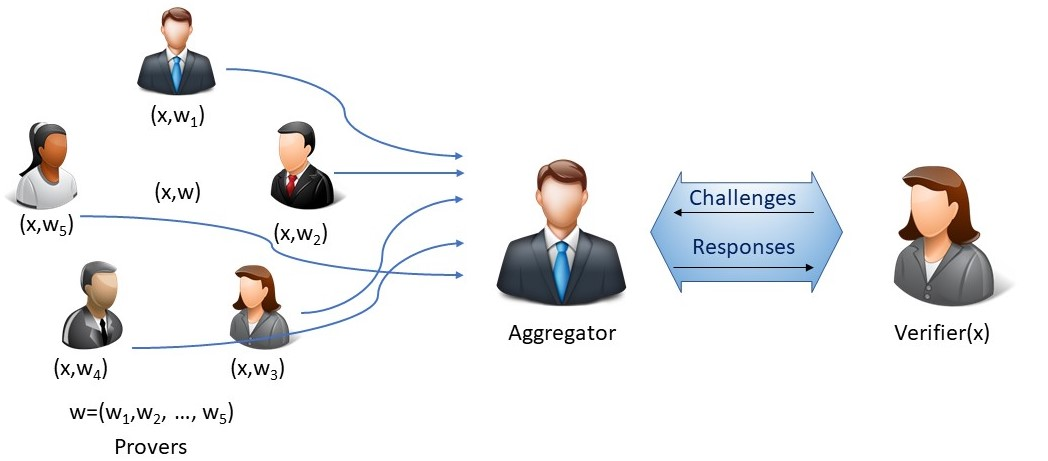
\includegraphics[width=0.9\linewidth]{DPZK.jpg}
%	\caption{Distributed Proof Generation}
%	\label{fig:DPZK}
%\end{figure}

\subsection{Related Notions}
Closely related to our notion is the work of \cite{EfficientTZ} which discusses threshold proofs. This work distributes the prover's side of interactive proofs of knowledge over multiple parties for: (i) improving the security against theft of the user's identity, (ii) improving robustness by ensuring that only a restricted size subset of the provers may be corrupted. The work of \cite{EfficientTZ} primarily captures sigma protocols without allowing interaction among the provers. Our definition captures a broader class of protocols via allowing interaction amongst the provers.  In other words, threshold proofs are a sub-class of the protocols we cater to. Also, other than increasing security via a decentralisation of the prover (or distributing prover's task), our goal is to capture scenarios where multiple provers would like to jointly prove a statement.  Our real-ideal world based definition is inline with MPC style definitions and is more powerful. Pedersen's PhD thesis \cite{Ped92} also defines distributed proofs. Our definition improves the notion of zero-knowledge in \cite{Ped92} where the security model is inherently restricted to a semi-honest collusion of the provers with the verifier. Also, \cite{Ped92} considers the provers' witnesses to always be secret shares of a ``global'' witness and hence the provers' witnesses are \textit{random} when the distributed proof generation begins. But, our definition allows for any distribution on the provers' witnesses, and this impacts some of our security proofs.


%We would like to finally point out that at many scenarios  
%In contrast to the definition in section ~\ref{sec:security model}, all the parties except for the verifier, in the execution of the protocol they may deviate arbitrarily, but the verifier is not allowed to deviate from the protocol. The reason behind considering a preposterously looking adversarial model is that we want to design a zkSNARK which is efficient, secure, publicly verifiable and distributed proof generation property. We know from \cite{}, any interactive honest (public coin) verifier can be transformed into Non-interactive zero-knowledge using \textit{Fiat–Shamir heuristic}. Here the verifier can be semi-honest, i.e., verifier will follow the protocol steps and sends all the challenges uniformly at random.
%-Start with corruption model and give a brief reasoning.
%.\pnote{Describe honest verifier}

\begin{comment}
If all the parties in $\Partyset$ are honest, then the protocol should return 1, this property is called \textbf{\textit{completeness}}.

In this setting, we have two types of corruption models, and that depends on which parties are corrupt:

-- Consider $I$, the set of all corrupt parties consists of all the provers in $\Partyset$, i.e., together they do not have a correct witness for $\stmt$, but they try to cheat in such a way so that the verifier outputs 1. What we want from the protocol is that such a scenario can happen with negligible probability. In other word, whenever in the protocol $\verifier$ outputs 1, then there must be a correct witness $\wit$ such that $\prover_i$ has $\wit_i$ for which $\wit = (\wit_1, \ldots, \wit_{\Num})$, with very high probability. This notion is called \textbf{\textit{proof of knowledge}}. 
	\begin{definition}
		Let $\Func_{\DPZK}$ is the functionality which is defined as ~\ref{func:DPZK} and let $\innp{\Pi}{V}$ is a $\DPZK$ $\Num$-party protocol involving $\Partyset$. We say that $\innp{\Pi}{V}$ realizes $\Func_{\DPZK}$ with computational proof of knowledge property if for every $\ppt$ real world adversary $\Adv$, corrupting at most all provers, there exists a $\ppt$ knowledge extractor $\extrac$ such that for every $\stmt \in L$, for which $\verifier$ outputs 1, $\extrac$ can extract a witness $(\wit_1, \ldots, \wit_{\Num})$ for which $\Func_{\DPZK}$ outputs 1.
	\end{definition}    
	
-- Consider $I$ consists of $\verifier$ and $t$ provers. That is, some of the provers may deviate from the protocol to gain additional information about the honest provers' secret; to achieve this, they may take additional help from $\verifier$'s view. We call a protocol $\innp{\Pi}{\verifier}$ has \textbf{\textit{zero knowledge under t-collusion}}($t$-ZKUC) property, if in this corruption model, corrupted provers and verifier whatever they can compute, the same thing can be computed from the functionality output of the functionality. 
	\begin{definition}
		Let $\Func_{\DPZK}$ is the functionality which is defined as ~\ref{func:DPZK} and let $\innp{\Pi}{V}$ is a $\DPZK$ $\Num$-party protocol involving $\Partyset$. We say that $\innp{\Pi}{V}$ realizes $\Func_{\DPZK}$ with computational zero knowledge under $t$-collusion property if for every $\ppt$ real world adversary $\Adv$, corrupting $I$, at most $t$ provers and verifier, then there exists a $\ppt$ simulator $\Sim$ such that for every $\stmt$, and $\{\wit_i : i\in [\Num]\}$, it holds that: 
		$$\Big\{\Ideal_{\Func_{\DPZK}, \Sim(\secparam),I}(\wit_1, \ldots, \wit_{\Num}) \Big\} \stackrel{c}{\approx} \Big\{ \Real_{\innp{\Pi}{\verifier}, \Adv(\secparam, \wit_T),I}(\wit_1, \ldots, \wit_{\Num}) \Big\}. $$
		Where $\wit_T$ is the input of the corrupt parties.
	\end{definition}

Note that if $I$ consists of the only verifier, then the view of the verifier should not reveal any information about neither the witness nor the inputs of the provers. This notion is called \textbf{\textit{zero knowledge}}, which is subsumed by the notion $t$-ZKUC.
\end{comment}

\section{Construction}




%\textbf{Encoding:} 
\paragraph{Encoding:}
Let, $x\in \mathbb{F}^{pml}$ %\mycomment{what is $pml$?add the details}
be the secret. We will encode $x$ to $U\in \mathbb{F}^{pmn}$ in the following way.\\
Let
%---------------------------------------

%---------------------------------------

Construct polynomials $p_{ij}(\cdot)$ %\mycomment{$p_{ij}(\cdot)$ use the cdot }
of degree $< s$ such that 
$ p_{ij}(\zeta_k)=x_{ijk} ~~\forall i\in [p], j\in [m], k\in [l]$.\\
Define:  $U$ %$\widetilde{U}$ \mycomment{$\widetilde{U}$ is not used below}
%---------------------------------------
$$U[i]=
\begin{bmatrix}
	p_{i1}(\eta_1) & p_{i1}(\eta_2) & \cdots & p_{i1}(\eta_n)\\
	p_{i2}(\eta_1) & p_{i2}(\eta_2) & \cdots & p_{i2}(\eta_n)\\
	\vdots\\
	p_{im}(\eta_1) & p_{im}(\eta_2) & \cdots & p_{im}(\eta_n)\\
\end{bmatrix}
$$
%---------------------------------------
and $U=[U[1], U[2], \cdots, U[p]]$.

So, $U$ is a box with $p$ slices and each slice has $m$ rows and $n$ columns.

\paragraph{Commitment:} Let $com$ be an homomorphic commitment scheme which commits a vector. Define:
%--------------------------------------- 
$$com(U)= [c_1,c_2,\cdots , c_p]^T=
 \begin{bmatrix} 
c[1,1] & c[1,2] & \cdots & c[1,n] \\
c[2,1] & c[2,2] & \cdots & c[2,n] \\
\vdots\\
c[p,1] & c[p,2] & \cdots & c[p,n]
\end{bmatrix}
=C$$
%---------------------------------------
where $c[i,k]=com([p_{i1}(\eta_k),p_{i2}(\eta_k),\cdots , p_{im}(\eta_k)]^T)$ and let $c$ is the Merkle tree root of $C$ where leaves are entries of $C$.

\paragraph{Protocol for Testing Interleaved:}
\textit{P} and \textit{V} does the following:

\begin{figure}[htb!]
	\centering
	\begin{tikzpicture}
		\node[block] (P) {\textit{P}};
		\node[block, right of = P, xshift=7cm] (V) {\textit{V}};
		\draw[->](1,-1)-- node[yshift=0.5em]{$c$}(7,-1);
		\draw[->](7,-2)-- node[yshift=0.5em]{$r\in_R \mathbb{F}^p$}(1,-2);
		\node[below of=P, xshift=-1em, yshift=-3em]{$\widetilde{U}=\sum\limits_{i\in [p]}r_i U[i]$};
		\node[below of=P, xshift=-1em, yshift=-5em]{$\tilde{c}=com(\widetilde{U})$};
		%---------------------
		\draw[->](1,-3.5)-- node[yshift=0.5em]{$\tilde{c}$}(7,-3.5);
		%\draw[->](7,-4.5)-- node[yshift=0.5em]{$Q\subset _R [n] : |Q|=t$}(1,-4.5);
		\draw[->](7,-4.5)-- node[yshift=0.5em]{$\gamma\in_R \mathbb{F}^m$}(1,-4.5);
		\node[below of=P, yshift=-16em]{$w=\gamma^T \widetilde{U}$};
		\draw[->](1,-5.5)-- node[yshift=0.6em]{$w$}(7,-5.5);
		\draw[->](7,-6.5)-- node[yshift=0.5em]{$Q\subset _R [n] : |Q|=t$}(1,-6.5);
		\draw[->](1,-7.5)-- node[yshift=0.6em]{$\widetilde{U}[k]$ with the randomness to commit it:$ k\in Q$}(7,-7.5);
		\draw[->](1,-7.5)-- node[yshift=-0.5em]{$C[k]: k \in Q$ and corresponding Merkle paths}(7,-7.5);
	\end{tikzpicture}
	\caption{Protocol for Testing Interleaved}
\end{figure}

\textit{P} and \textit{V} follows the protocol in Figure 1 and then
\textit{V} checks the following:
\begin{itemize}
	\item[(a)] Validation of $C[k]$ with respect to $c$.
	\item[(b)] $\tilde{c}_k = \sum\limits_{i\in[p]} r_ic_{ik}$ $\forall k\in Q$
	\item[(c)] $w\in L$, $L$ is the set of codewords.
	\item[(d)] $\sum\limits_{j\in [m]} \gamma_j \widetilde{U}[j,k] = w_k$ $\forall k\in Q'$
	\item[(e)] $open(\tilde{c}_k) = \widetilde{U}[k]$ $\forall k\in Q'$
\end{itemize}

\textbf{Completeness:} It is easy to see that if \textit{P} has correct witness, for any choice of $r, Q, \gamma, Q'$ of \textit{V}, \textit{P} can response for which \textit{V} accepts.\\

\textbf{Soundness:} The following lemma ensures the soundness:
%\textbf{Lemma}
 \begin{lemma} Suppose $d(U^*,L^{mp})>e$, where $e$ is some positive integer such that $e<\frac{d}{3}$\mycomment{(what is the bound of $e$)}, $U^*$ is not a correct encoding then any adversarial prover strategy succeeds with probability at most $(1-\frac{e}{2n})^{\kappa}+\frac{d}{|\mathbb{F}|}+neg(\kappa)$.
 \end{lemma}
 
 \begin{proof}
 	Let $\overline{U}= \sum\limits_{i\in[p]}r_iU^{*}[i]$.\\
	Then with probability $\geq 1-\frac{d}{|\mathbb{F}|}, \overline{U}$ satisfies $d(\overline{U},L^m)>e$.\\
	Let $\overline{c}$ be the commitment for $\overline{U}$, that implies $\overline{c}=r^T\overline{C}$, by the homomorphic property of the commitment scheme, where $\overline{C}$ is the commitment of $\overline{U}$.\\
	\textbf{Define: } Let $c,c'$ be two vectors, the distance between these two vectors is denoted by $d(c,c')$ and defined by the number of positions where $c$ and $c'$ differs.\\
	\textbf{case 1:} $d(\overline{c},\tilde{c})\geq \frac{e}{2}$ where $\tilde{c}= r^TC$, where $C$ is the commitment of $U$, nearest element of $U^*$ in $L^{mp}$.\\
	Prover's success probability $\leq \frac{\binom{n-e/2}{t}}{\binom{n}{t}}\approx(1-\frac{e}{2n})^t\approx(1-\frac{e}{2n})^k$ since $t=O(k)$\\
	\textbf{case 2:} $d(\overline{c},\tilde{c})< \frac{e}{2}$.\\
	Let, $\overline{\Delta}=\Delta(\overline{U}, L^m)$, positions where $\overline{U}$ is different from the nearest correct code slice.\\
	and let $\partial=\Delta(\overline{c},\tilde{c})$\\
	We have, $\overline{\Delta}>e$ and $\partial<\frac{e}{2}$, 
	$\Rightarrow |\overline{\Delta}\setminus \partial| \geq \frac{e}{2}$.\\
	Therefore, for $j\in \overline{\Delta}\setminus \partial$, $\overline{c}_j=\tilde{c}_j \Rightarrow \overline{U}[j]=\widetilde{U}[j]$\\
	Therefore probability of prover's success in the check (d) is $(1-\frac{e}{2n})^t\approx(1-\frac{e}{2n})^k$ since $t=O(k)$\\
	So the soundness error is $(1-\frac{e}{2n})^{\kappa}+\frac{d}{|\mathbb{F}|}+neg(\kappa)$.
 \end{proof}
 
 %\textbf{Zero knowledge:} The prover is sending $w$ to the verifier, so we want to modify $w$ in such a way that a correct $w$ should pass the check, but it should not reveal anything about $\widetilde{U}$, for that reason we will consider $\widetilde{U}$ to be a matrix of size $(m+1)\times n$, where the new row is a codeword.\\
% Now to hide $U$ from $\widetilde{U}$ we will blind by adjoining a new slice to $U$ of size $(m+1)\times n$, which will have weight 1, in computing $\widetilde{U}$. So, final modification in $U$ is $U[i]$ is a matrix of size $(m+1)\times n$ where first $m$ rows are same as defined above and the $(m+1)th$ row is all zeros, for all $i\in[p]$ and $U[p+1]$ is a random code slice of size $(m+1)\times n$.\\
 
 \textbf{Communication Complexity:} 
 \begin{itemize}
 	\item \underline{Proof Size}: constant size Merkle root, commitment vector with n components, with each component is of constant size, say $\lambda$, together $(n+1)\lambda$, $t$ many $C[j]$ and Merkle paths, size is $t(p.\lambda + \log n)$, $n$ sized vector $w$, $t$ many $\widetilde{U}[j]$ and randomness of total size $t(n+\alpha)$, where size of the randomness is $\alpha$.\\
	Therefore size of the proof is $\lambda(n+1)+t(p\lambda+\log n)+n+t(n+\alpha)= O(\sqrt[3]{|C|})$
	\item \underline{Verifier's Complexity}: $O(tm(M+E))$, where $M$ is the cost of multiplication and $E$ is the complexity of exponentiation. So, in this construction $O(\sqrt[3]{|C|})$ many cryptographic(elliptic curve) operations are required.
	\item \underline{Prover's complexity}: To construct commitment matrix $|C|$ may exponentiation, to construct $\widetilde{U}$, $|C|$ many multiplication, and to construct $w$, $mn$ many multiplication.\\
	So total complexity of the Prover is $mnM+|C|(M+E)=O(|C|(M+E))$
  \end{itemize}
 
\vspace*{50pt}
\paragraph{Protocol for checking Linear Constraint:} $x$ such that $Ax=b$ \\
\textit{P} and \textit{V} does the following:
\vspace*{40pt}
\begin{figure}[htb!]
	%\centering
	\begin{tikzpicture}
		\node[block] (P) {\textit{P}};
		\node[block, right of = P, xshift= 7cm] (V) {\textit{V}};
		\draw[->](1,-1)-- node[yshift=0.5em]{$c$}(7,-1);
		\draw[->](7,-2)-- node[yshift=0.5em]{$\overline{r}\in_R \mathbb{F}^{pml}$}(1,-2);
		\node[below of=P, yshift=-4em]{Define: $r=\overline{r}^TA$};
		\node[below of=P, yshift=-5.5em]{Construct polynomials $r_{ij}(.)$ of deg $< l$};
		\node[below of=P, yshift=-7.5em]{Define $q_j(.)=\sum\limits_{i\in[p]} r_{ij}(.).p_{ij}(.)$ $\forall j\in [m]$};
		\node[below of=P, yshift=-9em]{Define matrix $\overline{q}=(q_{ij})_{m\times n}$, where $q_{ij}=q_i(\eta_j)$};
		\node[below of=P, yshift=-10.5em]{Define $d_i=com([q_{1i},q_{2i},\cdots,q_{mi}]^T)$ $\forall i\in[h]$, $h=s+l-1$}; 
		\node[below of=P, yshift=-12em]{$T\in \mathbb{F}^{h\times n}$ such that$[p(\eta_1),\cdots,p(\eta_h)]T=[p(\eta_1),	\cdots,p(\eta_n)]$};
	%--------------------
		\draw[->](1,-7)-- node[yshift=1em]{$\{d_i:i\in[h]\}, q(.)=\sum\limits_{j\in [m]}q_j(.)$}(7,-7);
		\draw[->](7,-8)-- node[yshift=0.5em]{$Q\subset _R [n] : |Q|=t$}(1,-8);
		\draw[->](1,-9)-- node[yshift=0.5em]{$\overline{q}[k] \& C[k]: k \in Q$ and Merkle paths for $c$}(7,-9);
		\draw[->](7,-10)-- node[yshift=0.5em]{$Q'\subset _R [m] : |Q'|=t$}(1,-10);
		\draw[->](1,-11)-- node[yshift=0.5em]{$U[.,j,k]:j\in Q', k\in Q $ and randomness}(7,-11);
	\end{tikzpicture}
	\caption{Protocol for checking Linear Constraint}
\end{figure}

\textit{V} checks that:
\begin{itemize}
	\item[(a)] Validation of $C[k]$ with respect to $c$. 
	\item[(b)] $\sum\limits_{k\in [l]} q(\zeta_k)=\overline{r}^Tb$
	\item[(c)] Check $q(.)$ using $d_1,\cdots,d_h$: $<1,\overline{q}[j']>=q(\eta_{j'})\forall j'\in[h]$ as the inner product of the commitments should match with the commitment on the value $q(\eta_{j'})$. Using the idea of bullet proofs. Note that Verifier does not have $\overline{q}[j'] $ for all $j'\in[h]$ but still this check is possible using the commitments $d_1,\cdots, d_h$.
	\item[(d)] Reveal($\sum\limits_{j'\in [h]} T_{j'k} d_{j'})=\overline{q}[k] \forall k\in Q$
	\item[(e)] Check $U[.,j,k]$ with respect to $C[k]$ $\forall k\in Q,  j\in Q'$: $<e_j,U[i,.,k]>=U[i,j,k]$
	\item[(f)] $\sum\limits_{i\in[p]} r_{ij}(\eta_k) U[i,j,k]=\overline{q}[k]_j$ $\forall k\in Q$ and $j\in Q'$\\
\end{itemize}

\textbf{Completeness:} If the prover encodes the correct $x$ which satisfies $Ax=b$, then all the above checks will be passed, which ensures the completeness property.\\

\textbf{Soundness:} The following lemma ensures the soundness:

\begin{lemma}
	Let $e$ be a positive integer such that $e < \frac{d}{3}$. Suppose that a malformed $U^*$ is $e$-close to a codeword $U\in L^{mp}$ encoding $x\in \mathbb{F}^{pml}$ such that $Ax=b$. Then, for any malicious \textit{P} strategy, $U^*$ is rejected by \textit{V} except with at most $((e +k +l)/n)^{\kappa} +1/|\mathbb{F}|+neg(\kappa)$ probability.
\end{lemma}

\begin{proof}
	Since we assume that $Ax\neq b$, therefore $Pr_r[r^TAx=r^Tb]$ is at most $\frac{1}{|\mathbb{F}|}$.\\
	 Otherwise, \textit{P} must have sent a wrong $q'$, instead of $q$. Since, degree of $q'$ and $q$ can be at most $k+l-2$, as $q'$ is fixed after fixing the matrix $\overline{q}$, which is fixed and ensured to the verifier by providing $d_1,\cdots, d_h$. $q$ and $q'$ could be same in at most $k+l-2$ many indices of $\eta$. Let, $\overline{Q}$ is the set of indices where $q'$ and $q$ agree. and $E$ be the set of indices where $U$ and $U^*$ are different. Therefore, in check (f), prover fails if $k\in Q$ such that $k\notin \overline{Q}\cup E$. Therefore \textit{P} can cheat with probability at most $\frac{\binom{e+k+l-2}{t}}{\binom{n}{t}}\approx (\frac{e+k+l}{n})^t\approx (\frac{e+k+l}{n})^{\kappa}$.\\
	 Therefore soundness error is $(\frac{e+k+l}{n})^{\kappa}+\frac{1}{|\mathbb{F}|}+neg(\kappa)$, ($neg(\kappa)$ is due to the soundness probability of the commitment scheme).
\end{proof}

\textbf{Zero Knowledge:} %To achieve zero knowledge, modify $U$ in the following way, say $U'$: Set $U'$ of size $(p+1)\times (m+1)\times n$, $U'[i]=U[i]$ for the first $m$ rows and all zeros in the $(m+1)th$ row. Set $U'[p+1]$ zeros in all the positions in the first $m$ rows and put $u'$ in the $(m+1)th$ row, where $u'$ encodes to $v_1,\cdots, v_l$ such that $\sum\limits_{c\in[l]}v_c=0$. In this encoding, $q_{m+1}$ be the corresponding polynomial, let's call this $r_{blind}$, which has degree $<k+l-1$. so \textit{P} will send $q'(\cdot)=q(\cdot)+r_{blind}(\cdot)$, which will ensure the zero knowledge.\mycomment{(We need to blind two things (i) $q(\cdot)$ and (ii) $\overline{q}$, which consists of evaluation of $q_j$ on $\eta$'s)}\\

%To achieve zero knowledge, we need to blind two things (i) $q(\cdot)$ and (ii) $\overline{q}$, which consists of evaluation of $q_j$ on $\eta$'s. For to do that we are going to modify $U$.\\
%Define: $q'_j(\cdot)=q_j(\cdot)+r_{{blind}_j}(\cdot)$ $\forall j\in [m]$, where $r_{{blind}_j}(\cdot)$ are polynomials of degree $<k+l-1$ and $r_{{blind}_j}(\zeta_c)=0$ $\forall c\in[l], j\in [m]$.\\
%and finally, define $q(\cdot)= \sum\limits_{j\in[m]}q'_j(\cdot)+r_{blind}(\cdot)$, where $r_{blind}(\cdot)$ is polynomial of degree $<k+l-1$ and $r_{blind}(\zeta_c)=0$ $\forall c\in[l]$.\\
%So modify $U$ in the following way, say $U'$, Set $U'$ of size $(p+1)\times (m+1)\times n$, $U'[i]=U[i]$ for the first $m$ rows and all zeros in the $(m+1)th$ row. Set $U'[p+1](j,k)=r_{{blind}_j}(\eta_k)$ $\forall j\in[m], k\in [n]$ and $U'[p+1](m+1,k)=r_blind(\eta_k)$ $\forall k\in[n]$.\\
\textbf{Communication Complexity:}
\begin{itemize}
	\item \underline{Proof Size}: First \textit{P} sends Merkle root, which is of constant size, say $\lambda$,  then sends $(k+l-1)$ many commitments of constant size and $(k+l-1)$ many coefficients of $q$, therefore, $(\lambda+1)\times (k+l-1)$. $t\times m$ to send $t$ columns of $\overline{q}$ and $t \times p\lambda$ for $t$ columns of $C$, and for Merkle paths $t \times \log (pn)$. Finally $t^2$ many vectors from $U$ including the randomness to commit \textit{P} needs to send $t^2(p+\alpha)$. So, total size of the proof is $\sqrt[3]{|C|}$.
	\item \underline{Verifier's Complexity:} $l$ many polynomial evaluation of degree at most $(s+l-1)$, for that number of multiplication is $O(l(s+l-1))$,\\
	Checking commitments by IP using Bulletproofs, $(s+l-1)\sqrt{m}$ many exponentiations.\\
	$t(s+l-1)$ many multiplications.\\
	Checking commitments by IP using Bulletproofs, $t\sqrt{p}$ many exponentiations.\\
	and finally $tp$ many multiplications.\\
	In total: $l(s+l-1)+t(s+l-1)+tp$ multiplications and $(s+l-1)\sqrt{m}+t\sqrt{p}$ many exponentiations
	
	\item \underline{Prover's Complexity:}
	
\end{itemize}
%\vspace*{3.25cm}
\paragraph{Protocol for checking Quadratic Constraint:} $x,y,z$ suc that $x\odot y+a\odot z =b$\\
\textit{P} and \textit{V} does the following:
\begin{figure}[htb!]
	%\centering
	\begin{tikzpicture}
		\node[block] (P) {\textit{P}};
		\node[block, right of = P, xshift= 7cm] (V) {\textit{V}};
		\draw[->](1,-1)-- node[yshift=0.5em]{$c^x, c^y, c^z$}(7,-1);
		\draw[->](7,-2)-- node[yshift=0.5em]{$r\in_R \mathbb{F}^{p}$}(1,-2);
		\node[below of=P, yshift=-4.5em]{Define: $p_{ij}(.)=p^x_{ij}(.).p^y_{ij}(.)+p^a_{ij}(.).p^z_{ij}(.)-p^b_{ij}(.)$};
		\node[below of=P, yshift=-6.5em]{Define: $q_{j}(.)=\sum\limits_{i\in[p]} r_i.p_{ij}(.)$ $\forall j\in [m]$};
		\node[below of=P, yshift=-8em]{Define matrix $\overline{q}=(q_{jk})_{m\times n}$, where $q_{jk}=q_j(\eta_k)$};
		\node[below of=P, yshift=-9.5em]{Define $d_i=com([q_{1i},q_{2i},\cdots,q_{mi}]^T)$ $\forall i\in[h]$ $h=2s-1$};
		\node[below of=P, yshift=-11em]{$T\in \mathbb{F}^{h\times n}$ such that$[p(\eta_1),\cdots,p(\eta_h)]T=[p(\eta_1),	\cdots,p(\eta_n)]$ };
		\draw[->](1,-6)-- node[yshift=1em]{$\{d_i:i\in[h]\}$}(7,-6);
		\draw[->](7,-7)-- node[yshift=1em]{$\gamma \in_R \mathbb{F}^m$}(1,-7);
		\draw[->](1,-8)-- node[yshift=1em]{$q(.)=\sum\limits_{j\in[m]} \gamma_j.q_j(.)$}(7,-8);
		\draw[->](7,-9)-- node[yshift=0.5em]{$Q\subset _R [n] : |Q|=t$}(1,-9);
		\draw[->](1,-10)-- node[yshift=0.5em]{$\overline{q}[k] \& C^{\delta}[k]: k \in Q$ and Merkle paths for $c^{\delta}: 		\delta\in\{x,y,z\}$}(7,-10);
		\draw[->](7,-11)-- node[yshift=0.5em]{$Q'\subset _R [m] : |Q'|=t$}(1,-11);
		\draw[->](1,-12)-- node[yshift=0.5em]{$U^{\delta}[.,j,k]:j\in Q', k\in Q, \delta\in\{x,y,z\}$ and randomness}(7,-12);
	\end{tikzpicture}
\caption{Protocol for checking Quadratic constraint}
\end{figure}

\textit{V} checks that:
\begin{itemize}
	\item[(a)] Validation of $C^{\delta}[k]$ with respect to $c^{\delta}$, where $\delta\in\{x,y,z\}$. 
	\item[(b)] $\forall c\in[l], q(\zeta_c)=0$
	\item[(c)] Check $q(.)$ using $d_1,\cdots,d_h$: $<\gamma,\overline{q}[j']>=q(\eta_{j'})\forall j'\in[h]$ as the inner product of the commitments should match with the commitment on the value $q(\eta_{j'})$. Using the idea of bullet proofs. Note that Verifier does not have $\overline{q}[j'] $ for all $j'\in[h]$ but still this check is possible using the commitments $d_1,\cdots, d_h$.
	\item[(d)] Reveal($\sum\limits_{j'\in [h]} T_{j'k} d_{j'})=\overline{q}[k] \forall k\in Q$
	\item[(e)] Check $U^{\delta}[.,j,k]$ with respect to $C^{\delta}[k]$ $\forall k\in Q,  j\in Q'$: $<e_j,U^{\delta}[i,.,k]>=U^{\delta}[i,j,k]$, where $\delta\in\{x,y,z\}$. 
	\item[(f)] $\sum\limits_{i\in[p]} r_{i}[U^x[i,j,k].U^y[i,j,k]+U^a[i,j,k].U^z[i,j,k]-U^b[i,j,k]]=\overline{q}[k]_j$ $\forall k\in Q$ and $j\in Q'$\\
\end{itemize}

\textbf{Completeness:} If the prover encodes the correct $x,y,z$ which satisfy $x\odot y + a\odot z=b$, then all the above checks will be passed, which ensures the completeness property.\\

\textbf{Soundness:} The following lemma ensures the soundness:

\begin{lemma}
		
\end{lemma}

\textbf{Zero Knowledge:}

\textbf{Communication Complexity:}
%-------------------------------------------------------------------------------------
\section{Multi-Prover Setting}

Let, $P_1,P_2,\cdots,P_N$ provers are there. Let $w$ be the extended witness which is additively distributed and $w_{\nu}$ is the share of the witness of the $\nu$th party $\Rightarrow \sum\limits_{\nu \in [N]}w_{\nu}=w$\\
$P_{\nu}$ encodes $w_{\nu}$ in the following way:\\
Let $w_{\nu}\in \mathbb{F}^{pml}$, then we can write 

%---------------------------------------------------------------
$$w_{\nu} = 
\begin{bmatrix}
w_{\nu}[111] & w_{\nu}[112] & \cdots & w_{nu}[11l]\\
w_{\nu}[121] & w_{\nu}[122] & \cdots & w_{\nu}[12l]\\
\vdots\\
w_{\nu}[1m1] & w_{\nu}[1m2] & \cdots & w_{\nu}[1ml]\\
\vdots\\
w_{\nu}[pm1] & w_{\nu}[pm2] & \cdots & w_{\nu}[pml]
\end{bmatrix}
$$
%---------------------------------------------------------------
Construct `$pm$' many polynomials of degree $<s$ such that $p_{ij}(\zeta_c)=w_{\nu}[i,j,c]\forall i\in [p] j\in [m] c\in[l]$\\
Define: 
%---------------------------------------------------------------
$$U^{w_{\nu}}[i]=
\begin{bmatrix}
p_{i1}^{w_{\nu}}(\eta_1) & \cdots & p_{i1}^{w_{\nu}}(\eta_n)\\
p_{i2}^{w_{\nu}}(\eta_1) & \cdots & p_{i2}^{w_{\nu}}(\eta_n)\\
\vdots\\
p_{im}^{w_{\nu}}(\eta_1) & \cdots & p_{im}^{w_{\nu}}(\eta_n)\\
\end{bmatrix}
$$
%---------------------------------------------------------------
Define: $$U^{w_{\nu}}=[U^{w_{\nu}}[1] \cdots U^{w_{\nu}}[p]]$$\\
%---------------------------------------------------------------
Let $U=\sum\limits_{\nu \in [N]} U^{w_{\nu}}$.\\
Note that $U$ decodes to $w$. So let's call this $U^w$\\
Let $C^{w_{\nu}}, C^w$ be the commitment of $U^{w_{\nu}}, U^w$ respectively as mentioned in sectioin 1. Therefore by the homomorphic property of the commitment scheme $C^w=\sum\limits_{\nu \in [N]} C^{w_{\nu}}$.\\
%---------------------------------------------------------------
\paragraph{Protocol for Testing Interleaved:}
\textit{P}$\in \{P_1,\cdots, P_N\}$ is arbitrarily chosen.\\
\begin{figure}[htb!]
	\centering
	\begin{tikzpicture}
		\node[block] (A) {$P_{\nu}$};
		\node[block, right of = A, xshift=7cm] (P) {\textit{P}};
		\node[block, right of = P, xshift=7cm] (V) {\textit{V}};
		\draw[->](1,-1)-- node[yshift=1em]{$C^{w_{\nu}}$}(7,-1);
		\node[below of=P, xshift=-1em, yshift=-2em]{$C^w=\sum\limits_{\nu \in [N]}C^{w_{\nu}}$, $c$ is the Merkle root of $C^w$};
		\draw[->](8,-3)-- node[yshift=1em]{$c$}(15,-3);
		\draw[->](15,-4)-- node[yshift=0.5em]{$r\in_R \mathbb{F}^p$}(8,-4);
		\draw[->](7,-5)-- node[yshift=0.5em]{$r$}(1,-5);
		\node[below of=A, xshift=-1em, yshift=-5cm]{$\widetilde{U}^{w_{\nu}}=\sum\limits_{i\in [p]}r_i U^{w_{\nu}}[i]$};
		\draw[->](1,-6.5)-- node[yshift=0.6em]{$\widetilde{U}^{w_{\nu}}$}(7,-6.5);
		\node[below of=P, xshift=-1em, yshift=-17em]{$\widetilde{U}=\sum\limits_{\nu \in [N]}\widetilde{U}^{w_{\nu}}$};
		\node[below of=P, xshift=-1em, yshift=-18.5em]{$\tilde{c}=r^TC$};
		\draw[->](8,-8)-- node[yshift=0.5em]{$\tilde{c}$}(15,-8);
		\draw[->](15,-9)-- node[yshift=0.5em]{$\gamma \in_R \mathbb{F}^m$}(8,-9);
		\node[below of=P, xshift=-1em, yshift=-24em]{$w=\gamma^T \widetilde{U}$};
		\draw[->](8,-10)-- node[yshift=0.6em]{$w$}(15,-10);
		\draw[->](15,-11)-- node[yshift=0.5em]{$Q\subset _R [n] : |Q|=t$}(8,-11);
		\draw[->](8,-12)-- node[yshift=0.6em]{$\widetilde{U}[k]$ with the randomness to commit it:$ k\in Q$}(15,-12);
		\draw[->](8,-12)-- node[yshift=-0.5em]{$C[k]: k \in Q$ and corresponding Merkle paths}(15,-12);
	\end{tikzpicture}
	\caption{Protocol for Testing Interleaved}
\end{figure}

\textit{V} checks that:\\
\begin{itemize}
	\item[(a)] Validation of $C[k]$ with respect to the Merkle root $c$.
	\item[(b)] $\tilde{c}_k=\sum\limits_{i\in[p]}r_iC_{ik}$ $\forall k\in Q$
	\item[(c)] $w\in L$, $L$ is the set of codewords of size $\mathbb{F}^n$
	\item[(d)] $\sum\limits_{j\in [m]}\gamma_j \widetilde{U}_{jk}=w_k$ $\forall k\in Q$
	\item[(e)] $Open(\tilde{c}_k)=\widetilde{U}[k]$ $\forall k\in Q$
\end{itemize}

\paragraph{Protocol for Linear constraint:} Let $Ax=b$, where $A\in \mathbb{F}^{pml\times pml}$ and $b\in \mathbb{F}^{pml}$ are publicly known and $x$ is the secret which is additively distributed among the provers, say $x_{\nu}$ is the share of the $\nu$th prover.\\
$P_{\nu}$ encodes $x_{\nu}$ to $U^{\nu}$ and $C^{\nu}$ is the commitment of $U^{\nu}$.\\
\textit{P}$\in \{P_1,\cdots, P_N\}$ is arbitrarily chosen.\\
\begin{figure}[htb!]
	%\centering
	\begin{tikzpicture}
		\node[block] (A) {$P_{\nu}$};
		\node[block, right of = A, xshift=7cm] (P) {\textit{P}};
		\node[block, right of = P, xshift=6.5cm] (V) {\textit{V}};
		\draw[->](1,-1)-- node[yshift=1em]{$C^{\nu}$}(7,-1);
		\node[below of=P, xshift=-1em, yshift=-2em]{$C=\sum\limits_{\nu \in [N]}C^{\nu}$, $c$ is the Merkle root of $C$};
		\draw[->](8,-3)-- node[yshift=1em]{$c$}(15,-3);
		\draw[->](15,-4)-- node[yshift=0.5em]{$\overline{r}\in_R \mathbb{F}^{pml}$}(8,-4);
		\node[below of=P, xshift=-1em, yshift=-10em]{$r=\overline{r}^TA$};
		\draw[->](7,-5)-- node[yshift=0.5em]{$r$}(1,-5);
		\node[below of=A, yshift=-13em]{$q_j^{\nu}(\cdot)=\sum\limits_{i\in[p]}r_{ij}(\cdot)p_{ij}^{\nu}(\cdot)$ $\forall j\in[m]$};
		\node[below of=A, yshift=-15em]{$com(q_1(\eta_{j'}),\cdots,q_m(\eta_{j'}))=d_{j'}\forall j'\in [h]$};
		\node[below of=A, yshift=-17.5em]{$q^{\nu}(\cdot)=\sum\limits_{j\in [m]}q^{\nu}_j(\cdot)$};
		\draw[->](1,-8)-- node[yshift=0.6em]{$\{d_{j'}^{\nu}\}_{j'\in[h]}, q^{\nu}(\cdot)$}(7,-8);
		\node[below of=P, xshift=-1em, yshift=-22em]{$q(\cdot)=\sum\limits_{\nu \in [N]}q^{\nu}(\cdot)$};
		\node[below of=P, xshift=-1em, yshift=-24em]{$d_{j'}=\sum\limits_{\nu \in [N]}d_{j'}^{\nu}$};
		\draw[->](8,-10)-- node[yshift=0.6em]{$\{d_{j'}\}_{j'\in[h]}, q(\cdot)$}(15,-10);
		\draw[->](15,-11)-- node[xshift=-1em, yshift=0.5em]{$Q\subset _R [m]\times [n] : |Q|=t \& j_1\neq j_2$ and $k_1\neq k_2 \forall (j_1,k_1),(j_2,k_2)\in Q$}(8,-11);
		\draw[->](7,-12)-- node[xshift=-1em, yshift=0.5em]{$Q\subset _R [m]\times [n] : |Q|=t \& j_1\neq j_2$ and $k_1\neq k_2 \forall (j_1,k_1),(j_2,k_2)\in Q$}(1,-12);
		\draw[->](1,-13)-- node[yshift=0.6em]{$\{\{q^{\nu}_j(\eta_k)\}_{j\in[m]}:\forall k$, for some $j, (j,k)\in Q\}$}(7,-13);
		\node[below of=P, yshift=-36em]{$\overline{q}[k]=\{\sum\limits_{\nu \in [N]} q^{\nu}_j(\eta_k)\}_{j\in[m]}$};
		\draw[->](8,-15)-- node[yshift=0.6em]{$\overline{q}[k], C[k] \& U[\cdot,j,k] \forall k: (j,k)\in Q$}(15,-15);
		%\draw[->](8,-12)-- node[yshift=0.6em]{$\widetilde{U}[k]$ with the randomness to commit it:$ k\in Q$}(15,-12);
		%\draw[->](8,-12)-- node[yshift=-0.5em]{$C[k]: k \in Q$ and corresponding Merkle paths}(15,-12);				
	\end{tikzpicture}
	\caption{Protocol for Linear Constraint}
\end{figure}

%\mycomment{P sends Q to $P_{\nu}$ and from the reply P computes $\overline{q}[k]$}
\textit{V} checks that:\\
\begin{itemize}
	\item[(a)] Validation of $C[k]$ with respect to the Merkle root $c$.
	\item[(b)] $\sum\limits_{c\in[l]} q(\zeta_c)=\overline{r}^Tb$.
	\item[(c)] Check $q(\cdot)$ using $d_1,\cdots, d_h$ by InnerProduct argument using Bullet Proofs: $<1, \overline{q}[j']>= q(\eta_{j'})$ $\forall j'\in [h]$ where, commitment of $\overline{q}[j']$ is $d_{j'}$.
	\item[(d)] Reveal($\sum\limits_{j'\in[h]} T_{j'k}d_{j'})=q(\eta_k) \forall k\in[n]$, where $T$ is a public matrix of dimension $n\times h$ such that $T([p(\eta_1),\cdots,p(\eta_h)]^T)=([p(\eta_1),\cdots,p(\eta_n)]^T)$ for all polynomial of degree $<h$.
	\item[(e)] Check $U[\cdot,j,k]$ with respect to $C[k]$ $\forall (j,k)\in Q$ by InnerProduct argument using Bullet Proofs: $<e_j,U[i,\cdot,k]>=U[i,j,k]$.
	\item[(f)] $\sum\limits_{i\in [p]} r_{ij}(\eta_k)U[i,j,k]=\overline{q}[k]_j$ $\forall (j,k)\in Q$.
\end{itemize}

\paragraph{Protocol for quadratic constraint:} Let $x\odot y+a\odot z=b$, where $a,b$ are public and $x,y,z$ are secrets. $x_{\nu}, y_{\nu}, z_{\nu}$ are the shares of $P_{\nu}$. $P_{\nu}$ encodes $x_{\nu},y_{\nu},z_{\nu}$ to $U^{x_{\nu}},U^{y_{\nu}}, U^{z_{\nu}}$ respectively and computes the corresponding commitments i.e. $com(U^{x_{\nu}})=C^{x_{\nu}}, com(U^{y_{\nu}})=C^{y_{\nu}}, com(U^{z_{\nu}})=C^{z_{\nu}}$\\
$P_{\nu}$ constructs `$pm$' many polynomials $p^{(xy)_{\nu}}_{ij}(\cdot)$ such that $p^{(xy)_{\nu}}_{ij}(\cdot)= p^{x_{\nu}}_{ij}(\cdot)p^{y_{\nu}}_{ij}(\cdot)$. To do that use FFT and choose $\{\eta_1,\eta_2,\cdots,\eta_n\}$ accordingly, in particular, $n$th roots of unity and set $n\geq 2s-1$.\\
%Similarly, $P_{\nu}$ constructs polynomials $p^{(az)_{\nu}}_{ij}(\cdot)$ such that $p^{(az)_{\nu}}_{ij}(\cdot)= p^{a_{\nu}}_{ij}(\cdot)p^{z_{\nu}}_{ij}(\cdot)$.\\

\textit{P}$\in \{P_1,\cdots, P_N\}$ is arbitrarily chosen.\\
\begin{figure}[htb!]
	%\centering
	\begin{tikzpicture}
		\node[block] (A) {$P_{\nu}$};
		\node[block, right of = A, xshift=7cm] (P) {\textit{P}};
		\node[block, right of = P, xshift=6.5cm] (V) {\textit{V}};
		\draw[->](1,-1)-- node[yshift=1em]{$C^{\delta_{\nu}}, \delta\in \{x,y,z\}$}(7,-1);
		\node[below of=P, xshift=-1em, yshift=-2em]{$C^{\delta}=\sum\limits_{\nu \in [N]}C^{\delta_{\nu}}$, $c^{\delta}$ is the Merkle root of $C^{\delta}$, $\delta\in\{x,y,z\}$};
		\draw[->](8,-3)-- node[yshift=1em]{$c^{\delta}, \delta\in \{x,y,z\}$}(15,-3);
		\draw[->](15,-4)-- node[yshift=0.5em]{$r\in_R \mathbb{F}^{p}$}(8,-4);
		\draw[->](7,-5)-- node[yshift=0.5em]{$r$}(1,-5);
		\draw[->](1,-6)-- node[yshift=1em]{$p^{\nu}_{j}(\cdot)=\sum\limits_{i\in [p]}r_i[p^{(xy)_{\nu}}_{ij}(\cdot) + p^a_{ij}(\cdot)p^{z_{\nu}}_{ij}(\cdot)]$}(7,-6);
		\node[below of=P, xshift=-1em, yshift=-16em]{$q_j(\cdot)=\sum\limits_{\nu \in [N]} p^{\nu}_{j}(\cdot)- \sum\limits_{i\in [p]} r_ip^{b}_{ij}(\cdot)$};
		\node[below of=P, xshift=-1em, yshift=-18em]{Matrix $\overline{q}$ of size $m\times n$, $\overline{q}_{jk}= q_j(\eta_k)$};
		\node[below of=P, xshift=-1em, yshift=-20em]{$d_{j'}=com(\overline{q}[j'])$ $\forall j'\in [h]$};
		\draw[->](8,-9)-- node[yshift=1em]{$\{d_{j'}\}_{j'\in[h]}$}(15,-9);
		\draw[->](15,-10)-- node[yshift=1em]{$\gamma\in_R \mathbb{F}^m$}(8,-10);
		\node[below of=P, xshift=-1em, yshift=-28em]{Define: $q(\cdot)=\sum\limits_{j\in[m]}\gamma_jq_j(\cdot)$};
		\draw[->](8,-11.5)-- node[yshift=1em]{$q(\cdot)$}(15,-11.5);
		\draw[->](15,-12.5)-- node[xshift=-1em, yshift=1em]{$Q\subset _R [m]\times [n] : |Q|=t \& j_1\neq j_2$ and $k_1\neq k_2 \forall (j_1,k_1),(j_2,k_2)\in Q$}(8,-12.5);
		\draw[->](8,-13.5)-- node[xshift=-1em, yshift=1em]{$\overline{q}[k], C^{\delta}[k]$ and corresponding Merkle paths}(15,-13.5);
		\draw[->](8,-13.5)-- node[xshift=-1em, yshift=-1em]{$U^{\delta}[\cdot,j,k]$, where $\delta\in \{x,y,z\} \& \forall (j,k)\in Q$ }(15,-13.5);		
	\end{tikzpicture}
	\caption{Protocol for Quadratic Constraint}
\end{figure}
\FloatBarrier

\textit{V} checks that:\\
\begin{itemize}
	\item[(a)] Validation of $C^{\delta}[k]$ with respect to $c^{\delta}$, $\delta\in \{x,y,z\}$.
	\item[(b)] $q(\zeta_c)=0$ $\forall c\in [l]$.
	\item[(c)] Check using $d_1,\cdots, d_h$ using Inner Product argument by Bullet Proofs: $<\gamma, \overline{q}[j']>=q(\eta_{j'}) \forall j'\in [h]$.
	\item[(d)] Reveal($\sum\limits_{j'\in [h]} T_{j'k}d_{j'})= q(\eta_k) \forall k\in [n]$, where $T$ is a public matrix of dimension $n\times h$ such that $T([p(\eta_1),\cdots,p(\eta_h)]^T)=([p(\eta_1),\cdots,p(\eta_n)]^T)$ for all polynomial of degree $<h$.
	\item[(e)] Check $U^{\delta}[\cdot,j,k]$ with respect to $C^{\delta}[k]$ $\forall (j,k)\in Q$ by Inner Product argument using Bullet Proofs: $<e_j,U^{\delta}[i,\cdot,k]>=U^{\delta}[i,j,k]$.
	\item[(f)] $\sum\limits_{i\in [p]} r_i[U^x[i,j,k].U^y[i,j,k]+U^a[i,j,k].U^z[i,j,k]-U^b[i,j,k]]=\overline{q}[k]_j$ $\forall (j,k)\in Q$.
\end{itemize}
%--------------------------------------------------------------------------------------------
\section{Proof of size $|C|^{\frac{1}{\alpha}}$}
Here consider our extended witness $w\in \mathbb{F}^{pm_1m_2l}$. Encode it to $U^w$ in the same way as above, where size of $U$ is $p\times m_1m_2\times n$. Let, $m=m_1m_2$\\

\paragraph{Protocol for Testing Interleaved:}
\textit{P} and \textit{V} does the following:

\begin{figure}[htb!]
	\centering
	\begin{tikzpicture}
		\node[block] (P) {\textit{P}};
		\node[block, right of = P, xshift=7cm] (V) {\textit{V}};
		\draw[->](1,-1)-- node[yshift=0.5em]{$c$}(7,-1);
		\draw[->](7,-2)-- node[yshift=0.5em]{$r\in_R \mathbb{F}^p$}(1,-2);
		\node[below of=P, xshift=-1em, yshift=-3em]{$\widetilde{U}=\sum\limits_{i\in [p]}r_i U[i]$};
		\node[below of=P, xshift=-1em, yshift=-5em]{$\tilde{c}=com(\widetilde{U})$};
		%---------------------
		\draw[->](1,-3.5)-- node[yshift=0.5em]{$\tilde{c}$}(7,-3.5);
		%\draw[->](7,-4.5)-- node[yshift=0.5em]{$Q\subset _R [n] : |Q|=t$}(1,-4.5);
		\draw[->](7,-4.5)-- node[yshift=0.5em]{$\gamma\in_R \mathbb{F}^{m_1m_2}$}(1,-4.5);
		\node[below of=P, yshift=-11em]{$w=\gamma^T \widetilde{U}$};
		\draw[->](1,-5.5)-- node[yshift=0.6em]{$w$}(7,-5.5);
		\draw[->](7,-6.5)-- node[yshift=0.5em]{$Q\subset _R [n] : |Q|=t$}(1,-6.5);
		%\draw[->](1,-7.5)-- node[yshift=0.6em]{$\widetilde{U}[k]$ with the randomness to commit it:$ k\in Q$}(7,-7.5);
		\draw[->](1,-7.5)-- node[yshift=0.5em]{$C[k]: k \in Q$ and corresponding Merkle paths}(7,-7.5);
	\end{tikzpicture}
	\caption{Protocol for Testing Interleaved}
\end{figure}
\FloatBarrier

\textit{P} and \textit{V} follows the protocol in Figure 1 and then
\textit{V} checks the following:
\begin{itemize}
	\item[(a)] Validation of $C[k]$ with respect to $c$.
	\item[(b)] $\tilde{c}_k = \sum\limits_{i\in[p]} r_ic_{ik}$ $\forall k\in Q$
	\item[(c)] $w\in L$, $L$ is the set of codewords.
	\item[(d)] $\sum\limits_{j\in [m]} \gamma_j \widetilde{U}[j,k] = w_k$ $\forall k\in Q'$ Checking $\widetilde{U}$ with respect to it's commitment and $\gamma$ using inner product argument i.e. $<\gamma,  \widetilde{U}[k]>=w_k$ $\forall k\in[n]$
	%\item[(e)] $open(\tilde{c}_k) = \widetilde{U}[k]$ $\forall k\in Q'$
\end{itemize}

\textbf{Proof Size:} 
\begin{itemize} 
	\item constant size Merkle root
	\item $n$ sized vector $\tilde{c}$
	\item $n$ sized vector $w$
	\item $t$ many $p$ sized vector $C[k]:k\in Q$
	\item proof for inner product argument $O(log(m)$
\end{itemize}
So total size of the proof is $O(|C|^{\frac{1}{4}})$.

\textbf{Verifier's Complexity:}
\begin{itemize}
	\item Checking Merkle root
	\item $p$ multiplications: $pM$
	\item Multiplication by the Parity check matrix: $n^2M$
	\item Inner Product check :$m.E$
\end{itemize}
So total $mE+pM+n^2M$

\textbf{Prover's Complexity:}
\begin{itemize}
	\item Computing $C$, $|C|$ many exponentiation: $|C|.E$
	\item Computing Merkle root
	\item To compute $\widetilde{U}$, $|C|.M$ and to compute $\tilde{c}$, $p.n.M$
	\item To compute $w$, $m.n.M$
\end{itemize}
So total $|C|.E+|C|.M+p.n.M+m.n.M+h$, where $h$ is the complexit to compute the Merkle root.
%-----------------------------------------------------------
\paragraph{Protocol for checking Linear Constraint:} $x$ such that $Ax=b$ \\
\textit{P} and \textit{V} does the following:
\vspace*{40pt}
\begin{figure}[htb!]
	%\centering
	\begin{tikzpicture}
		\node[block] (P) {\textit{P}};
		\node[block, right of = P, xshift= 7cm] (V) {\textit{V}};
		\draw[->](1,-1)-- node[yshift=0.5em]{$c$}(7,-1);
		\draw[->](7,-2)-- node[yshift=0.5em]{$\overline{r}\in_R \mathbb{F}^{pm_1m_2l}$}(1,-2);
		\node[below of=P, yshift=-4em]{Define: $r=\overline{r}^TA$};
		\node[below of=P, yshift=-5.5em]{Construct polynomials $r_{ij}(.)$ of deg $< l$};
		\node[below of=P, yshift=-7.5em]{Define $q_j(.)=\sum\limits_{i\in[p]} r_{ij}(.).p_{ij}(.)$ $\forall j\in [m]$};
		\node[below of=P, yshift=-9em]{Define matrix $\overline{q}=(q_{jk})_{m_1m_2\times n}$, where $q_{jk}=q_j(\eta_k)$};
		\node[below of=P, yshift=-10.5em]{Define $d_{j'}=com([q_{1j'},q_{2j'},\cdots,q_{mj'}]^T)$ $\forall j'\in[h]$, $h=s+l-1$}; 
		\node[below of=P, yshift=-12em]{$T\in \mathbb{F}^{h\times n}$ such that$[p(\eta_1),\cdots,p(\eta_h)]T=[p(\eta_1),	\cdots,p(\eta_n)]$};
	%--------------------
		\draw[->](1,-7)-- node[yshift=1em]{$\{d_i:i\in[h]\}, q(.)=\sum\limits_{j\in [m]}q_j(.)$}(7,-7);
		\draw[->](7,-8)-- node[yshift=0.5em]{$Q\subset _R [n] : |Q|=t$}(1,-8);
		\draw[->](1,-9)-- node[yshift=0.5em]{$C[k]: k \in Q$ and Merkle paths for $c$}(7,-9);
		\draw[->](7,-10)-- node[yshift=0.5em]{$Q'\subset _R [m] : |Q'|=t$}(1,-10);
		\draw[->](1,-11)-- node[yshift=0.5em]{$U[.,j,k]:j\in Q', k\in Q $ and randomness}(7,-11);
	\end{tikzpicture}
	\caption{Protocol for checking Linear Constraint}
\end{figure}
\FloatBarrier

\textit{V} checks that:
\begin{itemize}
	\item[(a)] Validation of $C[k]$ with respect to $c$. 
	\item[(b)] $\sum\limits_{k\in [l]} q(\zeta_k)=\overline{r}^Tb$
	\item[(c)] Check $q(.)$ using $d_1,\cdots,d_h$: $<1,\overline{q}[j']>=q(\eta_{j'})\forall j'\in[h]$ as the inner product of the commitments should match with the commitment on the value $q(\eta_{j'})$. Using the idea of bullet proofs. Note that Verifier does not have $\overline{q}[j'] $ for all $j'\in[h]$ but still this check is possible using the commitments $d_1,\cdots, d_h$.
	%\item[(d)] Reveal($\sum\limits_{j'\in [h]} T_{j'k} d_{j'})=\overline{q}[k] \forall k\in Q$
	\item[(d)] Check $U[.,j,k]$ with respect to $C[k]$ $\forall k\in Q,  j\in Q'$: $<e_j,U[i,.,k]>=U[i,j,k]$
	\item[(e)] \textit{V} computes the value $\sum\limits_{j'\in[h]}T_{j'k}d_{j'}$ which is the commitment of the vector $\overline{q}[k]$ and also computes $\sum\limits_{i\in[p]} r_{ij}(\eta_k)U[i,j,k]$. Now use Inner Product argument i.e. $<e_j,\overline{q}[k]>=\sum\limits_{i\in[p]} r_{ij}(\eta_k)U[i,j,k]$ $\forall j\in Q', k\in Q$.
\end{itemize}
\textbf{Proof Size:}
\begin{itemize}
	\item Constant size Merkle root.
	\item $h$ many constants for $d_1,\cdots, d_h$ and $h$ coefficients for the polynomial, $O(h)$.
	\item $t$ many $C[k]$ and corresponding Merkle paths, total size: $t.p+ t\log(pn)$
	\item $t$ many $U[\cdot,j,k]$ and randomness: $O(t.p)$.
	\item Proof for Inner Product argument $O(\log(m))$
\end{itemize}
In total $O(|C|^{\frac{1}{4}})$

\textbf{Verifier's Complexity:} 
\begin{itemize}
	\item Checking Merkle roots.
	\item $l$ polynomial evaluations $(s+l-1).l.M$
	\item Inner Product check by the verifier: $O(m.E)$
	\item $(s+l-1).M+p.M+|C|.M+\log m. E$
\end{itemize}
So total $(s+l-1).l.M+ m.E+(s+l-1).M+p.M+|C|.M+\log m.E$


\textbf{Prover's Complexity:}
 To compute $C$ matrix, Prover needs to do $|C|$ many exponentiation and that is dominating term in his computation.
%-----------------------------------------------------------
\paragraph{Protocol for checking Quadratic Constraint:} $x,y,z$ suc that $x\odot y+a\odot z =b$\\
\textit{P} and \textit{V} does the following:
\begin{figure}[htb!]
	%\centering
	\begin{tikzpicture}
		\node[block] (P) {\textit{P}};
		\node[block, right of = P, xshift= 7cm] (V) {\textit{V}};
		\draw[->](1,-1)-- node[yshift=0.5em]{$c^x, c^y, c^z$}(7,-1);
		\draw[->](7,-2)-- node[yshift=0.5em]{$r\in_R \mathbb{F}^{p}$}(1,-2);
		\node[below of=P, yshift=-4.5em]{Define: $p_{ij}(.)=p^x_{ij}(.).p^y_{ij}(.)+p^a_{ij}(.).p^z_{ij}(.)-p^b_{ij}(.)$};
		\node[below of=P, yshift=-6.5em]{Define: $q_{j}(.)=\sum\limits_{i\in[p]} r_i.p_{ij}(.)$ $\forall j\in [m]$};
		\node[below of=P, yshift=-8em]{Define matrix $\overline{q}=(q_{jk})_{m_1m_2\times n}$, where $q_{jk}=q_j(\eta_k)$};
		\node[below of=P, yshift=-9.5em]{Define $d_{j'}=com([q_{1j'},q_{2j'},\cdots,q_{mj'}]^T)$ $\forall j'\in[h]$ $h=2s-1$};
		\node[below of=P, yshift=-11em]{$T\in \mathbb{F}^{h\times n}$ such that$[p(\eta_1),\cdots,p(\eta_h)]T=[p(\eta_1),	\cdots,p(\eta_n)]$ };
		\draw[->](1,-6)-- node[yshift=1em]{$\{d_i:i\in[h]\}$}(7,-6);
		\draw[->](7,-7)-- node[yshift=1em]{$\gamma \in_R \mathbb{F}^m$}(1,-7);
		\draw[->](1,-8)-- node[yshift=1em]{$q(.)=\sum\limits_{j\in[m]} \gamma_j.q_j(.)$}(7,-8);
		\draw[->](7,-9)-- node[yshift=0.5em]{$Q\subset _R [n] : |Q|=t$}(1,-9);
		\draw[->](1,-10)-- node[yshift=0.5em]{$C^{\delta}[k]: k \in Q$ and Merkle paths for $c^{\delta}: \delta\in\{x,y,z\}$}(7,-10);
		\draw[->](7,-11)-- node[yshift=0.5em]{$Q'\subset _R [m] : |Q'|=t$}(1,-11);
		\draw[->](1,-12)-- node[yshift=0.5em]{$U^{\delta}[.,j,k]:j\in Q', k\in Q, \delta\in\{x,y,z\}$ and randomness}(7,-12);
	\end{tikzpicture}
\caption{Protocol for checking Quadratic constraint}
\end{figure}
\FloatBarrier

\textit{V} checks that:
\begin{itemize}
	\item[(a)] Validation of $C^{\delta}[k]$ with respect to $c^{\delta}$, where $\delta\in\{x,y,z\}$. 
	\item[(b)] $\forall k\in[l], q(\zeta_k)=0$
	\item[(c)] Check $q(.)$ using $d_1,\cdots,d_h$: $<\gamma,\overline{q}[j']>=q(\eta_{j'})\forall j'\in[h]$ as the inner product of the commitments should match with the commitment on the value $q(\eta_{j'})$. Using the idea of bullet proofs. Note that Verifier does not have $\overline{q}[j'] $ for all $j'\in[h]$ but still this check is possible using the commitments $d_1,\cdots, d_h$.
	%\item[(d)] Reveal($\sum\limits_{j'\in [h]} T_{j'k} d_{j'})=\overline{q}[k] \forall k\in Q$
	\item[(d)] Check $U^{\delta}[.,j,k]$ with respect to $C^{\delta}[k]$ $\forall k\in Q,  j\in Q'$: $<e_j,U^{\delta}[i,.,k]>=U^{\delta}[i,j,k]$, where $\delta\in\{x,y,z\}$. 
	\item[(e)] \textit{V} computes the value $\sum\limits_{j'\in[h]}T_{j'k}d_{j'}$, which is the commitment of the vector$\overline{q}[k]$ and also computes$\sum\limits_{i\in[p]} r_i[U^{x}[i,j,k].U^y[i,j,k]+U^{a}[i,j,k].U^z[i,j,k]-U^{b}[i,j,k]] =R[i,j,k]$. Now use Inner Product argument i.e. $<e_j,\overline{q}[k]>=R[i,j,k]$ $\forall j\in Q', k\in Q$.\\
\end{itemize}

\textbf{Proof Size:}
\begin{itemize}
	\item Constant size Merkle root $c$.
	\item $d_1,\cdots, d_h$: $O(h)$.
	\item To send the polynomial $q(\cdot)$, $2s-1$ many coefficients are needed to be send.
	\item $t$ many $C[k]$, $t.p$
	\item $t$ many $U[\cdot,j,k]$, $t.p$
	\item Proof for Inner product argument: $\log m$
\end{itemize}
In total $O(h+2s-1+t.p+\log(m) = O(|C|^{\frac{1}{4}})$

\textbf{Verifier's Complexity:}
\begin{itemize}
	\item Checking Merkle roots.
	\item $l$ polynomial evaluations: $(2s-1).l.M$
	\item Checking using Inner Product arguments $O(m.E)$
	\item $(2s-1).M+t.p.M$
\end{itemize}
So total complexity $O(|C|^{\frac{1}{2}}. E + |C|^{\frac{1}{2}}. M)$

\textbf{Prover's Complexity:}
 To compute $C$ matrix, Prover needs to do $|C|$ many exponentiation and that is dominating term in his computation.

	
\end{document}